\chapter{TÌM HIỂU VỀ PHẦN MỀM ALTIUM DESIGNER}
    \section{Tìm hiểu về phần mềm Altium Designer}
        Altium Designer là một trong những phần mềm chuyên ngành cho phép thiết kế mạch điện tử PCB (Printed Circuit Board). Altium Designer là một phần mềm mạnh với nhiều tính năng. Một số tính năng cơ bản của phần mềm Altium Designer có thể kể đến như sau:
        \begin{itemize}
            \item Giao diện thiết kế, quản lý và chỉnh sửa thân thiện, dễ dàng biên dịch, quản lý file, quản lý phiên bản cho các tài liệu thiết kế.
            \item Hỗ trợ mạnh mẽ cho việc thiết kế tự động, đi dây tự động theo thuật toán tối ưu, phân tích lắp ráp linh kiện. Hỗ trợ việc tìm các giải pháp thiết kế hoặc chỉnh sửa mạch, linh kiện, netlist có sẵn từ trước theo các tham số mới.
            \item Mở, xem và in các file thiết kế mạch dễ dàng với đầy đủ các thông tin linh kiện, netlist, dữ liệu bản vẽ, kích thước, số lượng…
            \item Hệ thống các thư viện linh kiện phong phú, chi tiết và hoàn chỉnh bao gồm tất cả các linh kiện nhúng, số, tương tự…
            \item Đặt và sửa đối tượng trên các lớp cơ khí, định nghĩa các luật thiết kế, tùy chỉnh các lớp mạch in, chuyển từ schematic sang PCB, đặt vị trí linh kiện trên PCB.
            \item Mô phỏng mạch PCB 3D, đem lại hình ảnh mạch điện trung thực trong không gian 3 chiều, hỗ trợ MCAD-ECAD, liên kết trực tiếp với mô hình STEP, kiểm tra khoảng cách cách điện, cấu hình cho cả 2D và 3D.
            \item Hỗ trợ thiết kế PCB sang FPGA và ngược lại.
        \end{itemize}
        \begin{figure}[H]
            \centering
            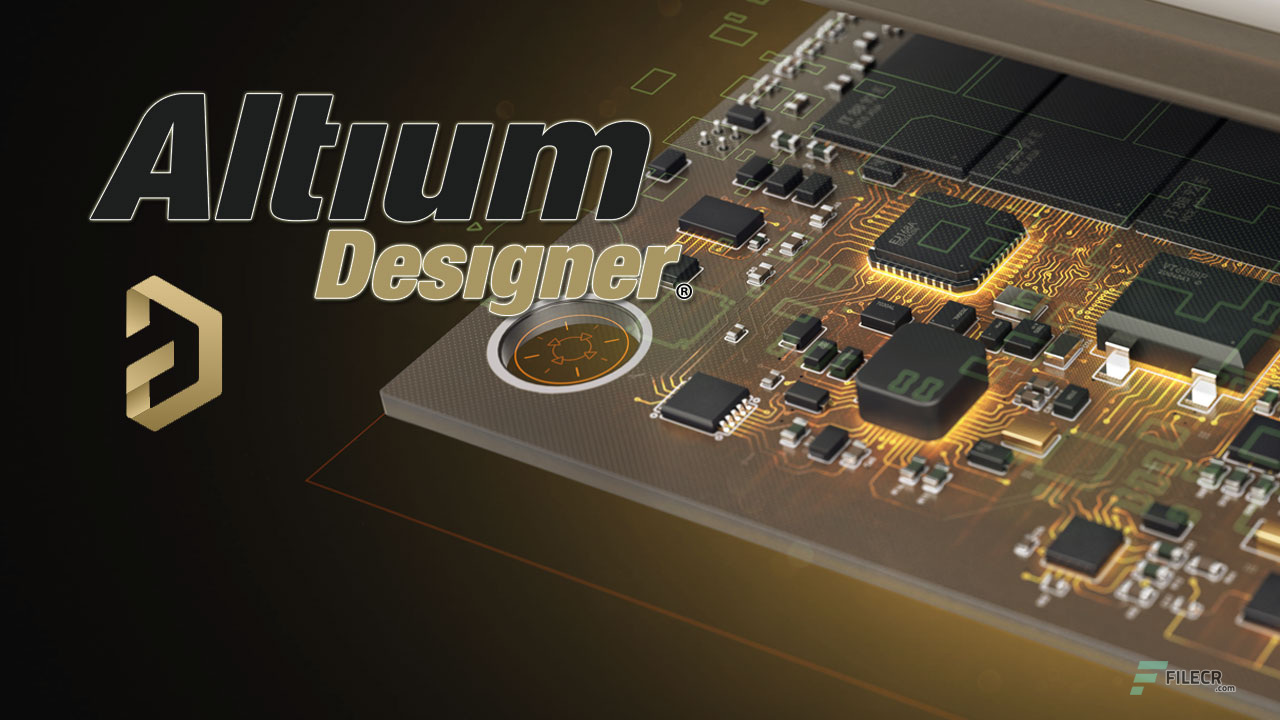
\includegraphics[width=0.6\textwidth]{pictures/altium.png}
            \caption{Phần mềm Altium Designer}
            \label{fig:altium}
        \end{figure}
        \cleardoublepage
    \section{Trình tự thiết kế mạch bằng phần mềm Altium Designer}
        \begin{enumerate}
            \item Thiết kế sơ đồ nguyên lí
            \item Lựa chọn các linh kiện phù hợp
            \item Lựa chọn các chân linh kiện để chuyển sang mạch in
            \item Update mạch nguyên lý sang mạch in
            \item Lựa chọn kích thước mạch in, giới hạn mạch in và thiết lập lớp phủ đất
            \item Sắp xếp các vị trí các loại linh kiện như điện trở, tụ điện, IC,…
            \item Đặt luật đi dây, các lỗ via, khoảng cách giữa các linh kiện, lỗ và dây
            \item Đi dây trên mạch và phủ đồng
            \item Kiểm tra toàn mạch
        \end{enumerate}
        \begin{figure}[H]
            \centering
            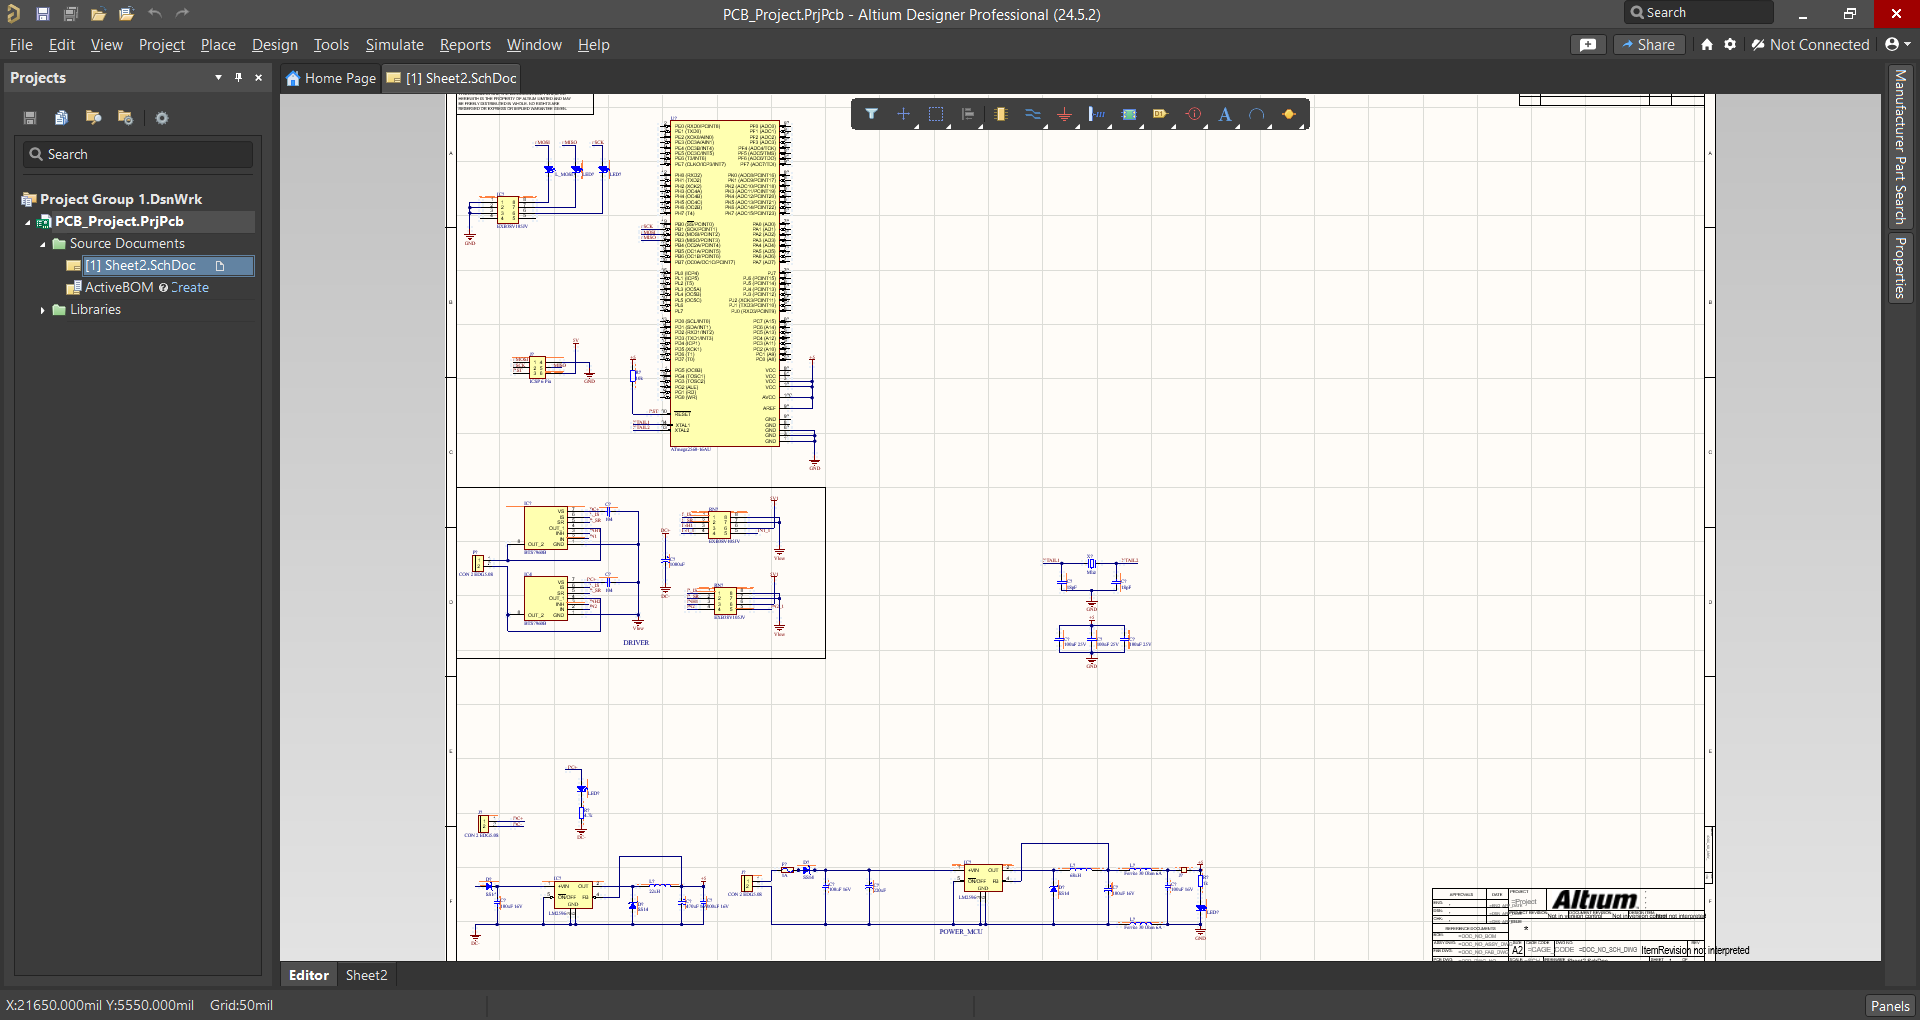
\includegraphics[width=1\textwidth]{pictures/workspacealtium.png}
            \caption{Giao diện làm việc của phần mềm Altium Designer}
            \label{fig:workspacealtium}
        \end{figure}
        \cleardoublepage
    \section{Sơ đồ nguyên lý}
        \subsection{Sơ lược về sơ đồ nguyên lý}
            Sơ đồ nguyên lý trong mạch điện tử là một biểu đồ biểu diễn các thành phần của
            mạch điện và cách chúng được kết nối với nhau. Mục tiêu là để mô tả chức năng của
            mạch một cách rõ ràng và dễ hiểu. Các thành phần phổ biến trong sơ đồ nguyên lý của
            mạch điện tử bao gồm:
            \begin{itemize}
                \item Điện trở (Resistor): Ký hiệu bằng hình chữ nhật hoặc zigzag. Điện trở được sử dụng để giới hạn dòng điện hoặc phân chia điện áp.
                \item Tụ điện (Capacitor): Ký hiệu bằng hai đường thẳng song song. Tụ điện lưu trữ và phóng điện năng.
                \item Cuộn cảm (Inductor): Ký hiệu bằng một loạt các vòng xoắn. Cuộn cảm lưu trữ năng lượng trong từ trường khi dòng điện chạy qua.
                \item Điốt (Diode): Ký hiệu bằng một tam giác và một vạch đứng. Điốt cho phép dòng điện chạy theo một chiều duy nhất.
                \item Transistor:
                \begin{itemize}
                    \item NPN: Ký hiệu bằng một mũi tên chỉ ra ngoài từ đường nối giữa base và emitter.
                    \item PNP: Ký hiệu bằng một mũi tên chỉ vào trong.
                \end{itemize}
                \item IC (Integrated Circuit): Ký hiệu bằng một hình chữ nhật với nhiều chân ra. IC chứa nhiều linh kiện điện tử tích hợp bên trong.
                \item Nguồn điện (Power Supply): Ký hiệu bằng hai đường thẳng song song, với một đường dài hơn (dương) và một đường ngắn hơn (âm).
            \end{itemize}
        \subsection{Ví dụ về sơ đồ nguyên lý}
            \begin{figure}[H]
                \centering
                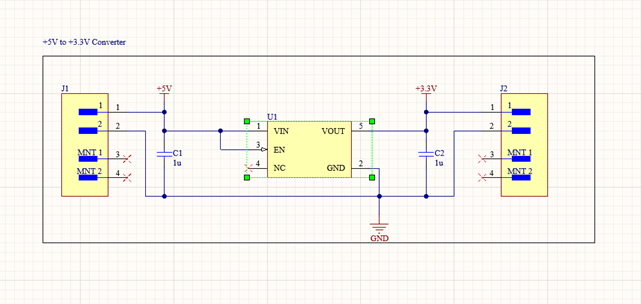
\includegraphics[width=1\textwidth]{pictures/sch1.png}
                \caption{Sơ đồ nguyên lý mạch chuyển đổi điện áp}
                \label{fig:sodonguyenly}
            \end{figure}
            \begin{figure}[H]
                \centering
                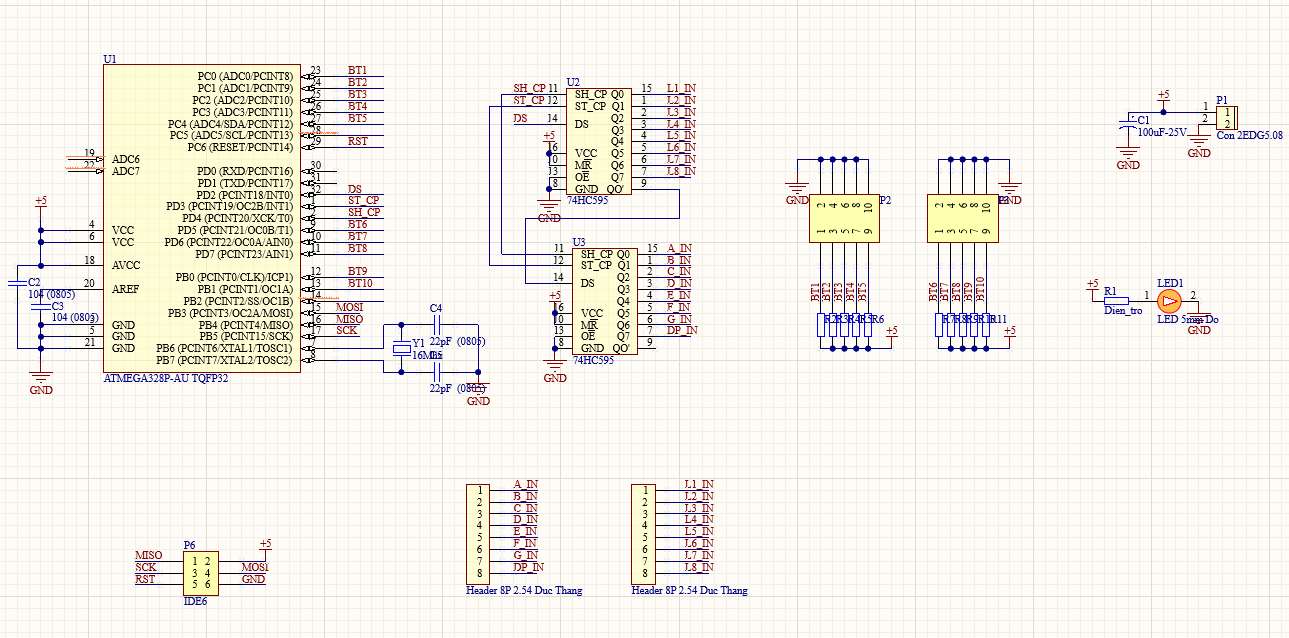
\includegraphics[width=1\textwidth]{pictures/sch2.png}
                \caption{Sơ đồ nguyên lý mạch điều khiển LED 7 đoạn}
                \label{fig:sodonguyenly}
            \end{figure}
            \begin{figure}[H]
                \centering
                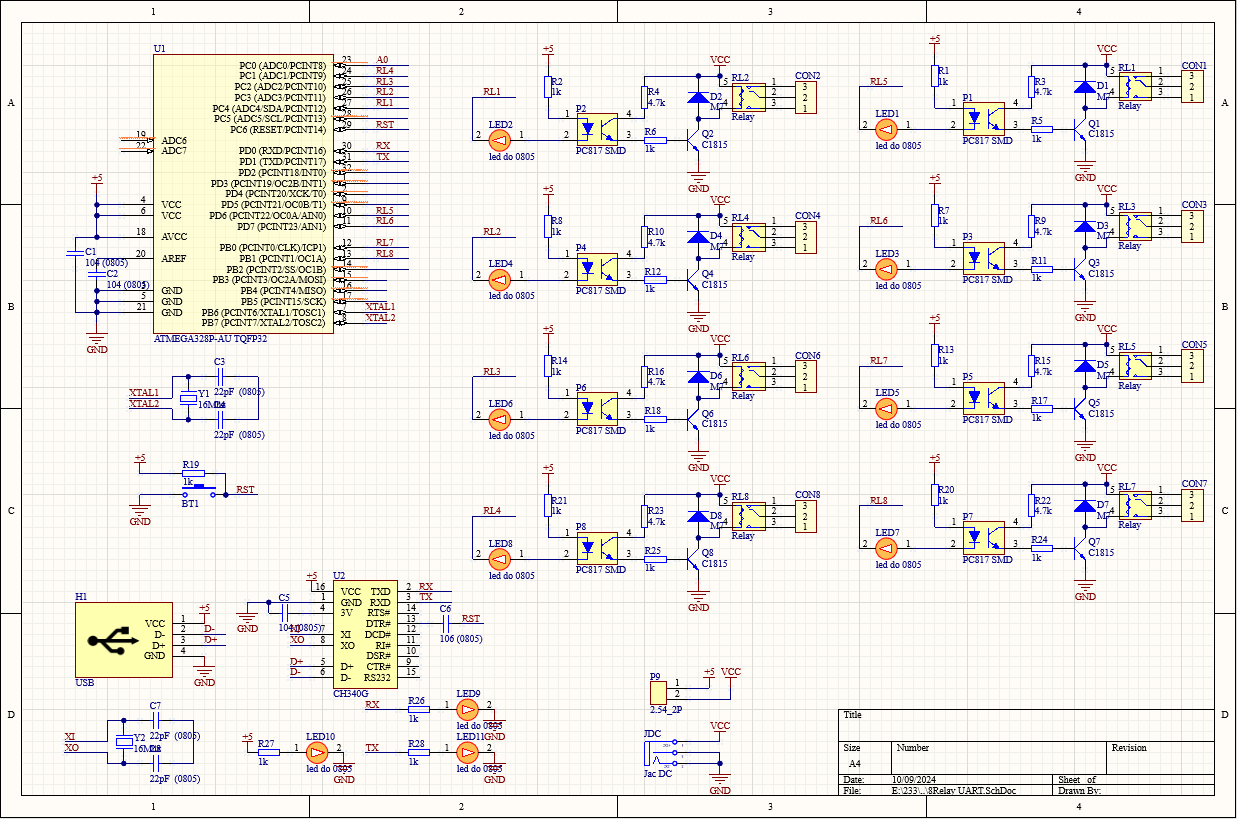
\includegraphics[width=1\textwidth]{pictures/sch3.png}
                \caption{Sơ đồ nguyên lý mạch điều khiển 8 relay}
                \label{fig:sodonguyenly}
            \end{figure}
            \begin{figure}[H]
                \centering
                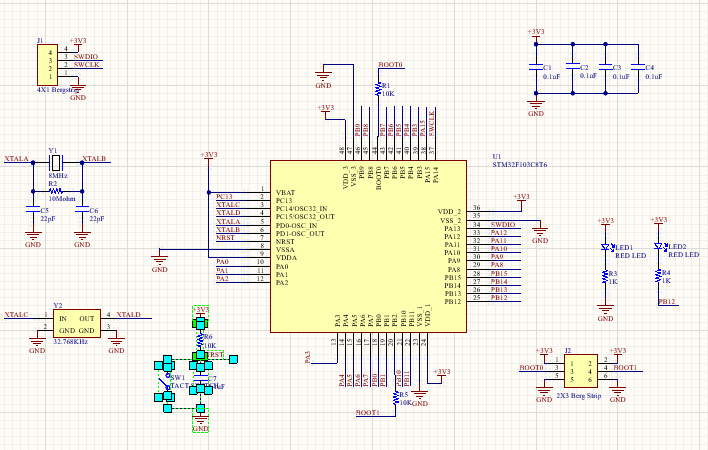
\includegraphics[width=1\textwidth]{pictures/sch4a.png}
                \caption{Sơ đồ nguyên lý mạch STM32F103C8T6 phần điều khiển}
                \label{fig:sodonguyenly}
            \end{figure}
            \begin{figure}[H]
                \centering
                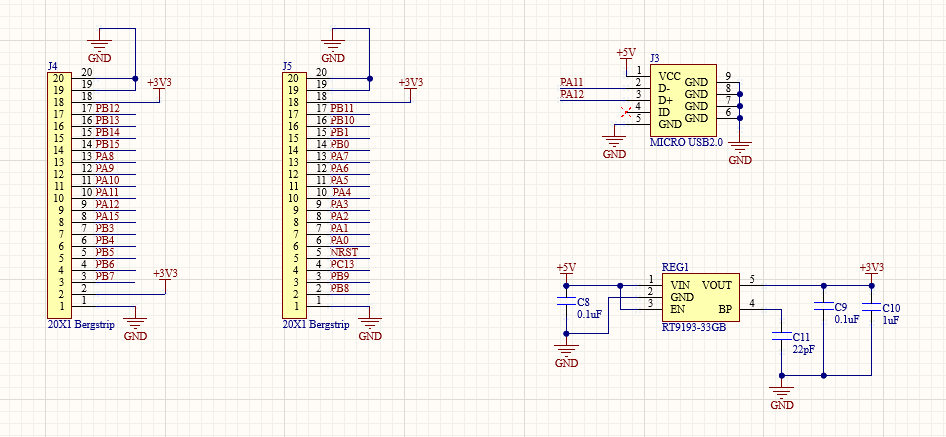
\includegraphics[width=1\textwidth]{pictures/4b.png}
                \caption{Sơ đồ nguyên lý mạch STM32F103C8T6 phần kết nối}
                \label{fig:sodonguyenly}
            \end{figure}
            \begin{figure}[H]
                \centering
                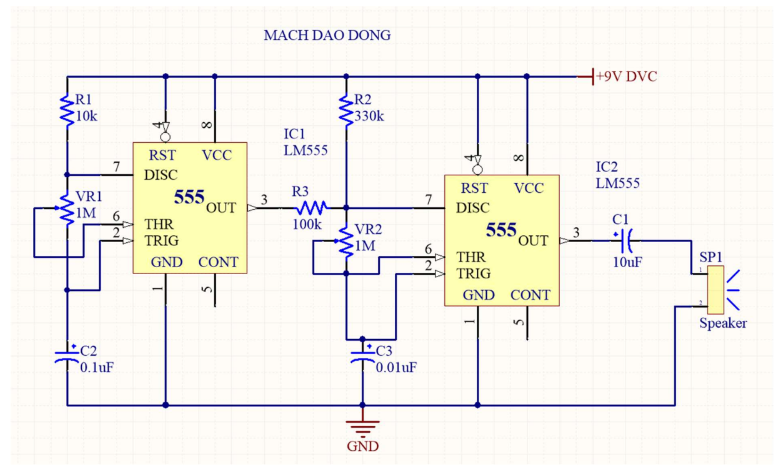
\includegraphics[width=1\textwidth]{pictures/sch5.png}
                \caption{Sơ đồ nguyên lý mạch dao động}
                \label{fig:sodonguyenly}
            \end{figure}
            \cleardoublepage
    \section{Mạch in PCB}
        \subsection{Sơ lược về mạch in PCB}
            Sơ đồ mạch in (PCB - Printed Circuit Board) là một bản vẽ chi tiết mô tả các
            thành phần và kết nối điện tử trên một bảng mạch. Để thiết kế một sơ đồ mạch in PCB,
            bạn cần phải thực hiện các bước cơ bản sau: 
            \begin{itemize}
                \item Xác định yêu cầu:
                \begin{itemize}
                    \item Xác định các thành phần cần thiết cho mạch.
                    \item Định rõ các yêu cầu về điện áp, dòng điện, và tần số.
                \end{itemize}
                \item Thiết kế sơ đồ nguyên lý (schematic):
                \begin{itemize}
                    \item Vẽ sơ đồ nguyên lý để biểu diễn các thành phần điện tử và kết nối giữa chúng.
                    \item Sử dụng phần mềm thiết kế mạch điện tử như Eagle, KiCad, Altium Designer,...
                \end{itemize}
                \item Chuyển sơ đồ nguyên lý thành sơ đồ mạch in (PCB layout):
                \begin{itemize}
                    \item Sử dụng phần mềm thiết kế PCB để tạo ra bố trí mạch in từ sơ đồ nguyên lý.
                    \item Đặt các thành phần trên bảng mạch sao cho tối ưu hóa không gian và đảm bảo hiệu quả kết nối điện.
                \end{itemize}
                \item Route các đường mạch:
                \begin{itemize}
                    \item Kết nối các chân của các thành phần bằng các đường mạch trên bảng PCB.
                    \item Đảm bảo các đường mạch không bị chồng chéo và tuân theo quy tắc thiết kế.
                \end{itemize}
                \item Kiểm tra và xác nhận thiết kế:
                \begin{itemize}
                    \item Kiểm tra sơ đồ mạch in để đảm bảo không có lỗi.
                    \item Sử dụng các công cụ kiểm tra DRC (Design Rule Check) để đảm bảo tuân thủ các quy tắc thiết kế.
                \end{itemize}
                \item Xuất file Gerber:
                \begin{itemize}
                    \item Xuất các file Gerber từ phần mềm thiết kế PCB để gửi đến nhà sản xuất PCB.
                    \item File Gerber là định dạng tiêu chuẩn được sử dụng trong sản xuất PCB.
                \end{itemize}
                \item Sản xuất PCB:
                \begin{itemize}
                    \item Gửi các file Gerber đến nhà sản xuất PCB để họ tạo ra bảng mạch thực tế.
                    \item Sau khi sản xuất, kiểm tra bảng mạch để đảm bảo chất lượng.
                \end{itemize}
            \end{itemize}
        \subsection{Ví dụ về mạch in PCB}
            \begin{figure}[H]
                \centering
                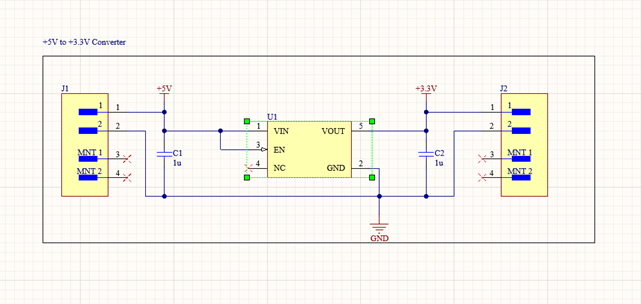
\includegraphics[width=1\textwidth]{pictures/sch1.png}
                \caption{Sơ đồ nguyên lý mạch chuyển đổi điện áp}
                \label{fig:sodonguyenly}
            \end{figure}
            \begin{figure}[H]
                \centering
                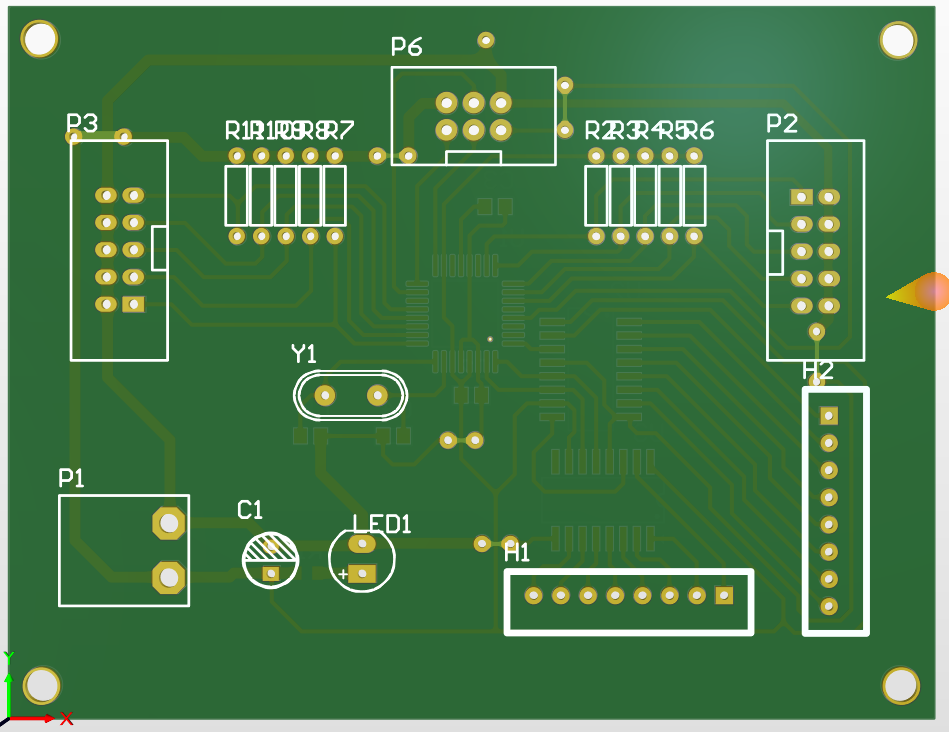
\includegraphics[width=1\textwidth]{pictures/pcb1.png}
                \caption{Mặt trước mạch điều khiển LED 7 đoạn}
                \label{fig:hbridge}
            \end{figure}
            \begin{figure}[H]
                \centering
                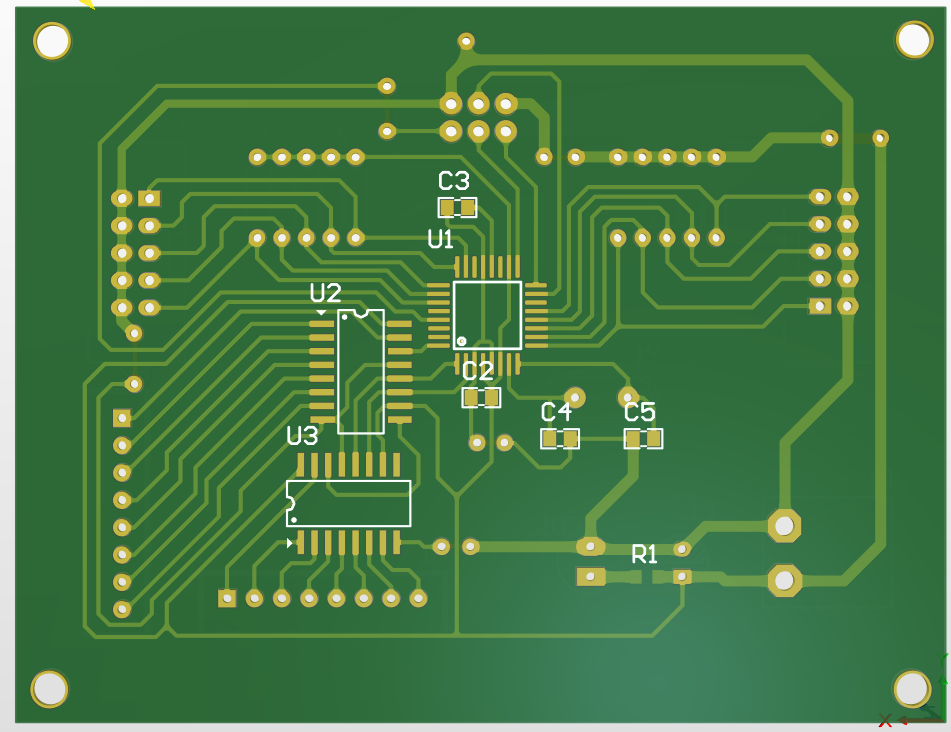
\includegraphics[width=1\textwidth]{pictures/pcb2.png}
                \caption{Mặt sau mạch điều khiển LED 7 đoạn}
                \label{fig:hbridge}
            \end{figure}
            \begin{figure}[H]
                \centering
                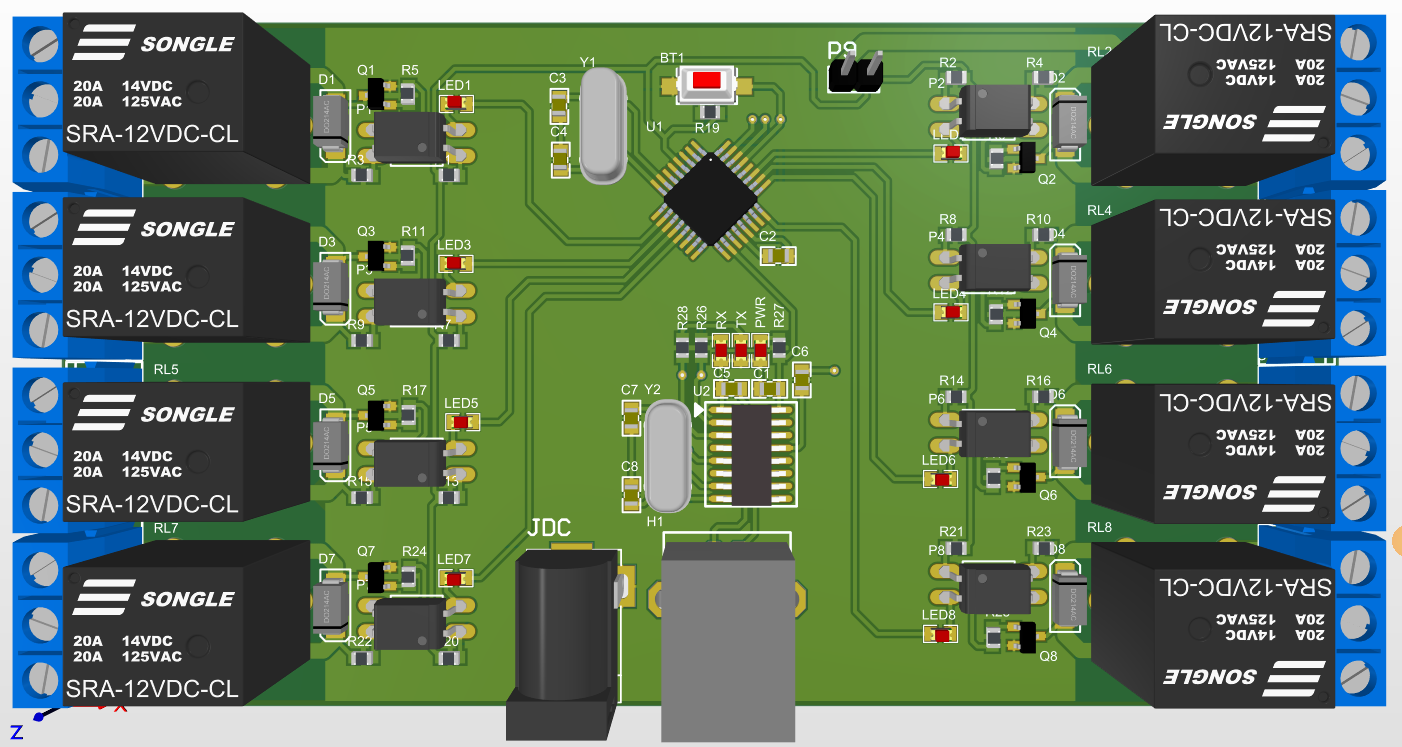
\includegraphics[width=1\textwidth]{pictures/pcb3.png}
                \caption{Mạch điều khiển 8 relay}
                \label{fig:hbridge}
            \end{figure}
            \begin{figure}[H]
                \centering
                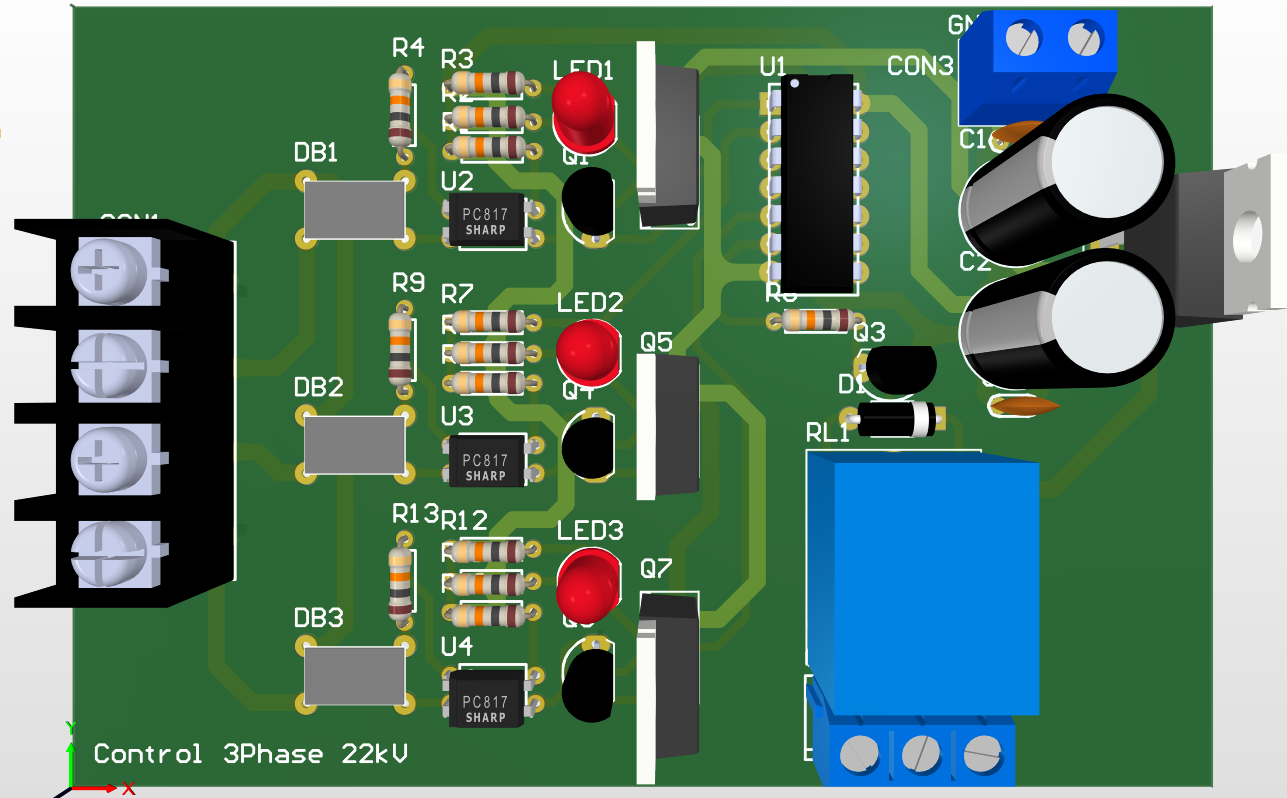
\includegraphics[width=1\textwidth]{pictures/pcb4.png}
                \caption{Mạch điều khiển 3 pha}
                \label{fig:hbridge}
            \end{figure}
            \begin{figure}[H]
                \centering
                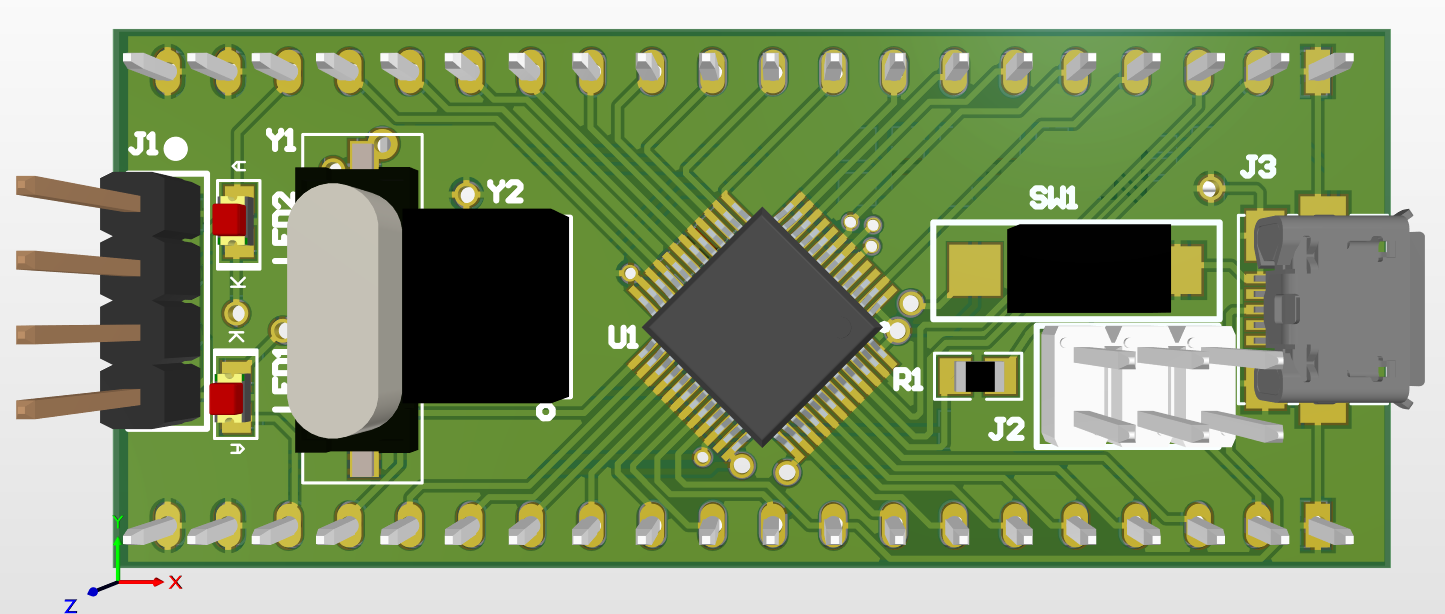
\includegraphics[width=1\textwidth]{pictures/pcb5.png}
                \caption{Mạch STM32F103C8T6}
                \label{fig:hbridge}
            \end{figure}
            \cleardoublepage
        \section{TẠO THƯ VIỆN SCHEMATIC VÀ PCB 3D}
            \subsection{Trình tự tạo thư viện schematic}
                Bước 1: Chọn File/New/Library để tạo thư viện mới.
                \begin{figure}[H]
                    \centering
                    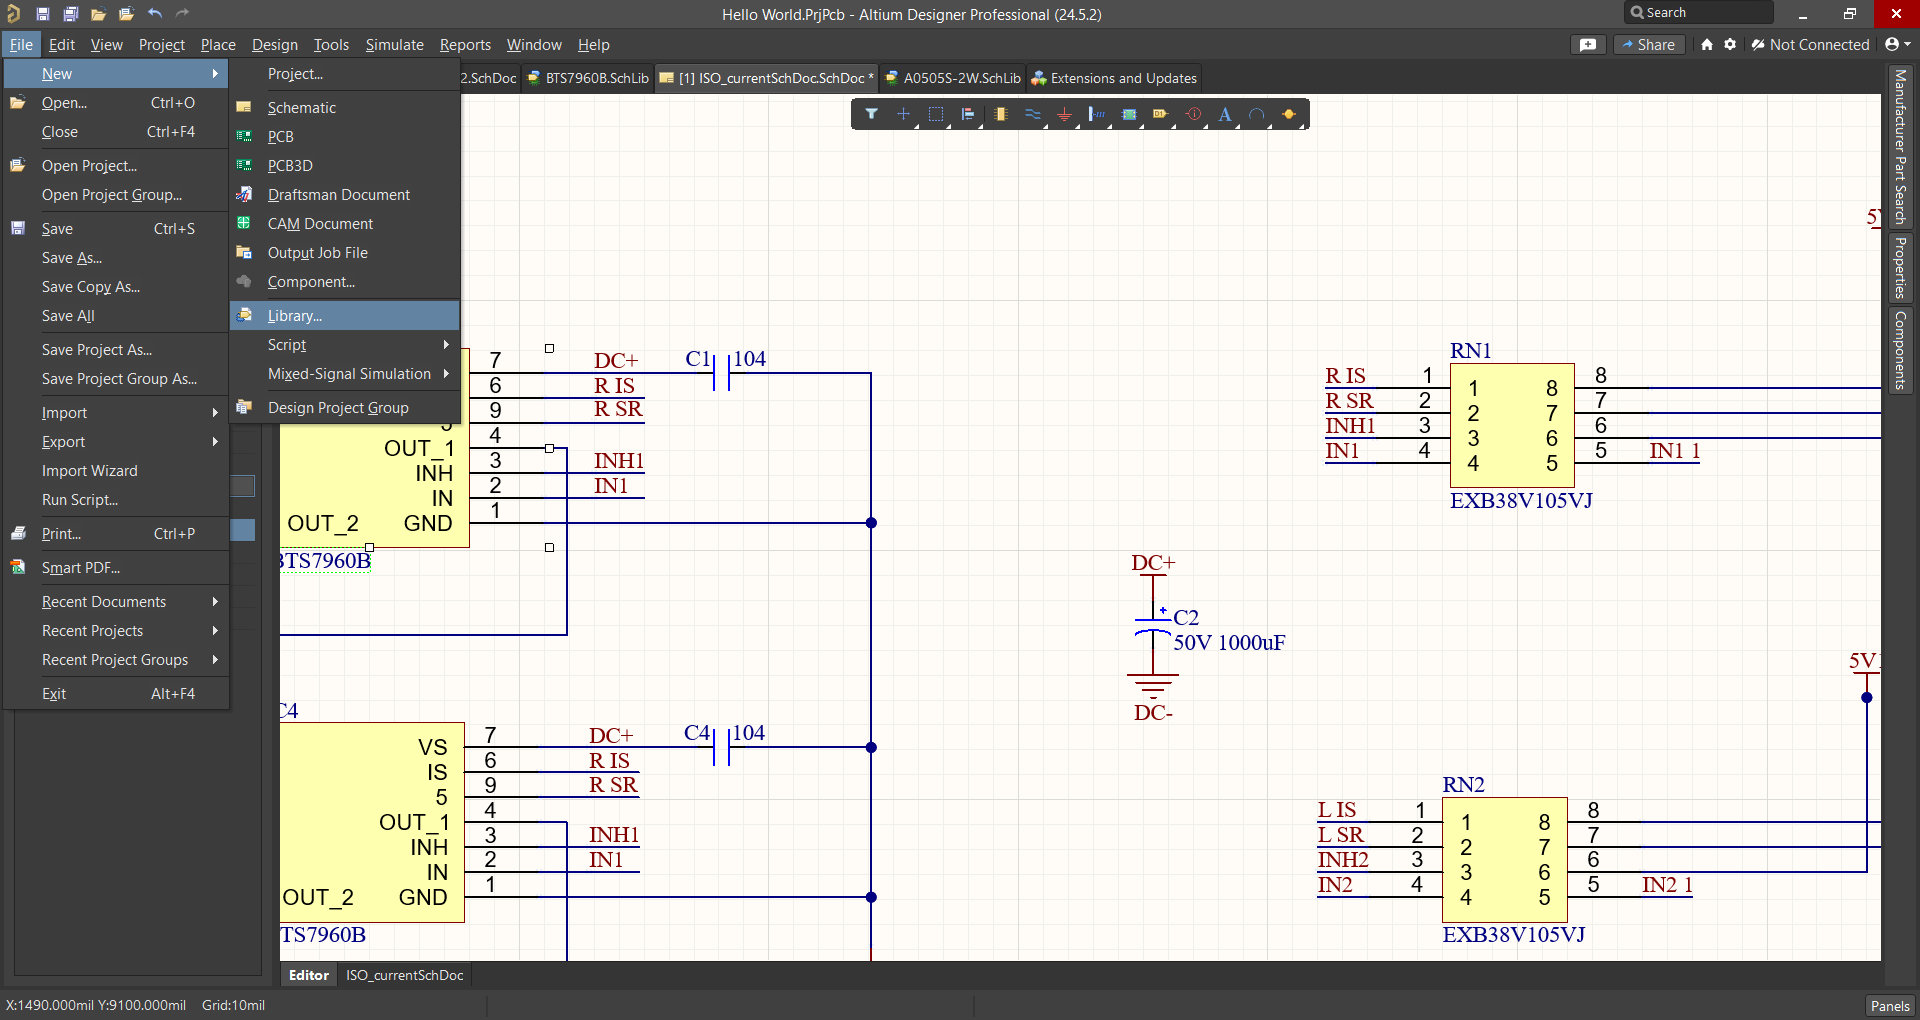
\includegraphics[width=1\textwidth]{pictures/ch3.1.png}
                \end{figure}
                Bước 2: Chọn Schematic Library và nhấn Create.
                \begin{figure}[H]
                    \centering
                    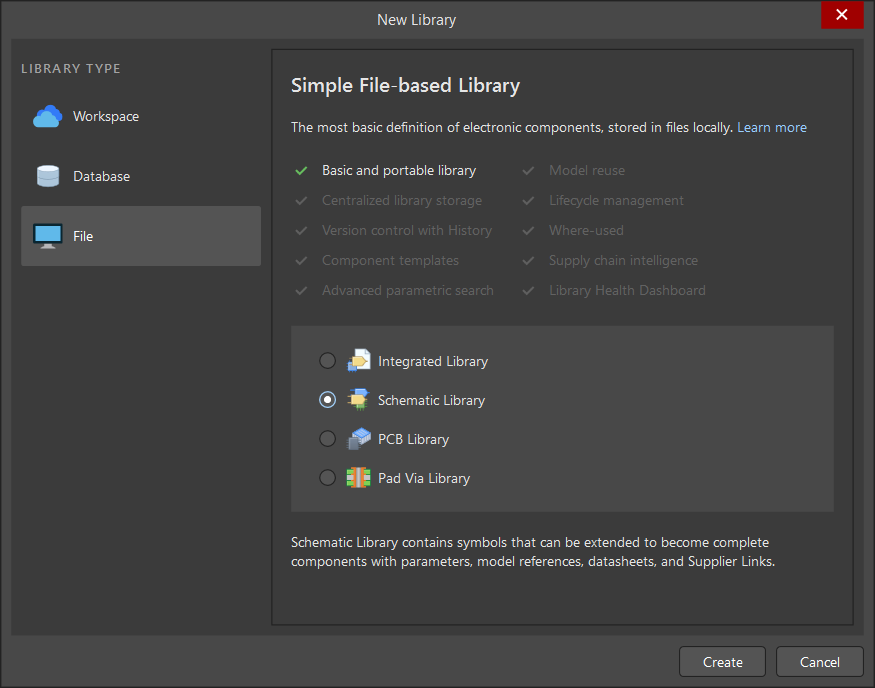
\includegraphics[width=0.8\textwidth]{pictures/ch3.2.png}
                \end{figure}
                Bước 3: Vẽ khối và đặt các chân theo hướng dẫn của datasheet.
                \begin{figure}[H]
                    \centering
                    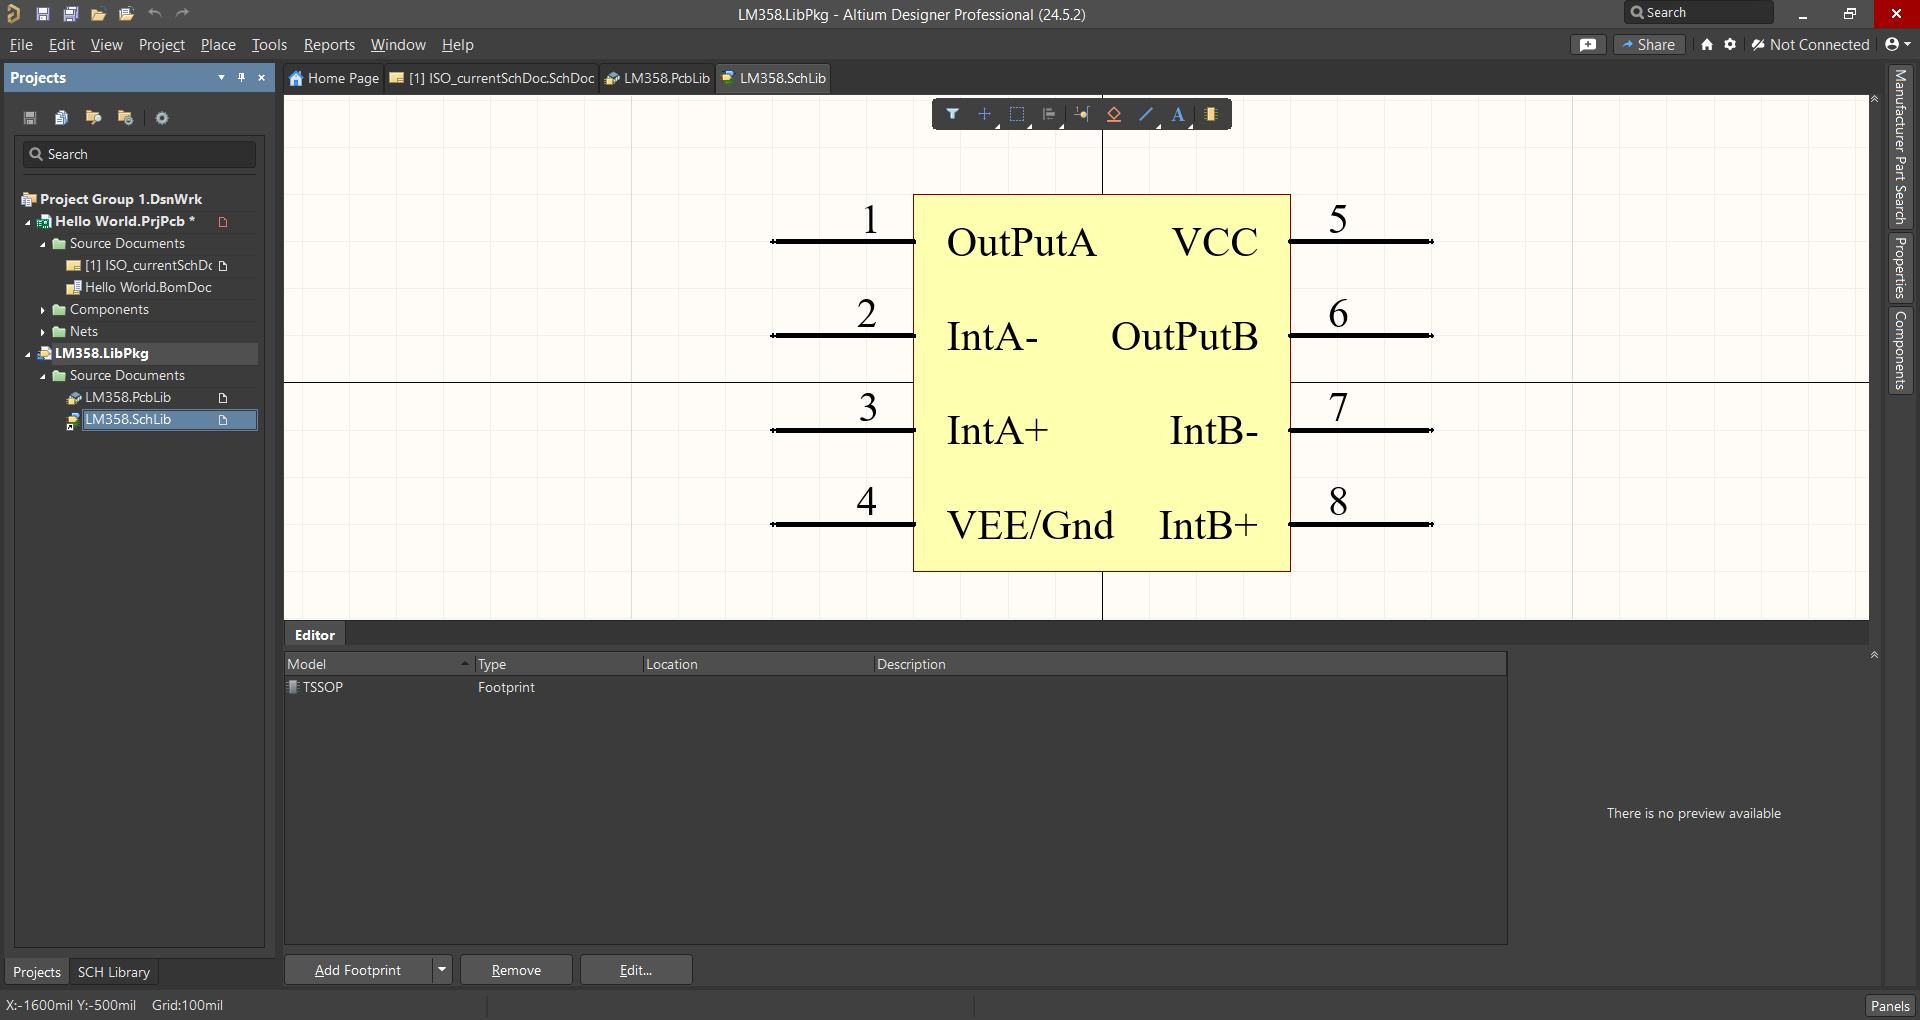
\includegraphics[width=1\textwidth]{pictures/ch3.3.png}
                \end{figure}
                Bước 4: Đặt tên cho thư viện và lưu lại.\\
            \subsection{Trình tự tạo thư viện PCB }
                \textbf{Ví dụ: Tạo thư viện fPCB 3D cho LM358 SOP8.}\\
                Bước 1: Chọn File/New/Library để tạo thư viện mới.\\
                Bước 2: Chọn PCB Library và nhấn Create.
                \begin{figure}[H]
                    \centering
                    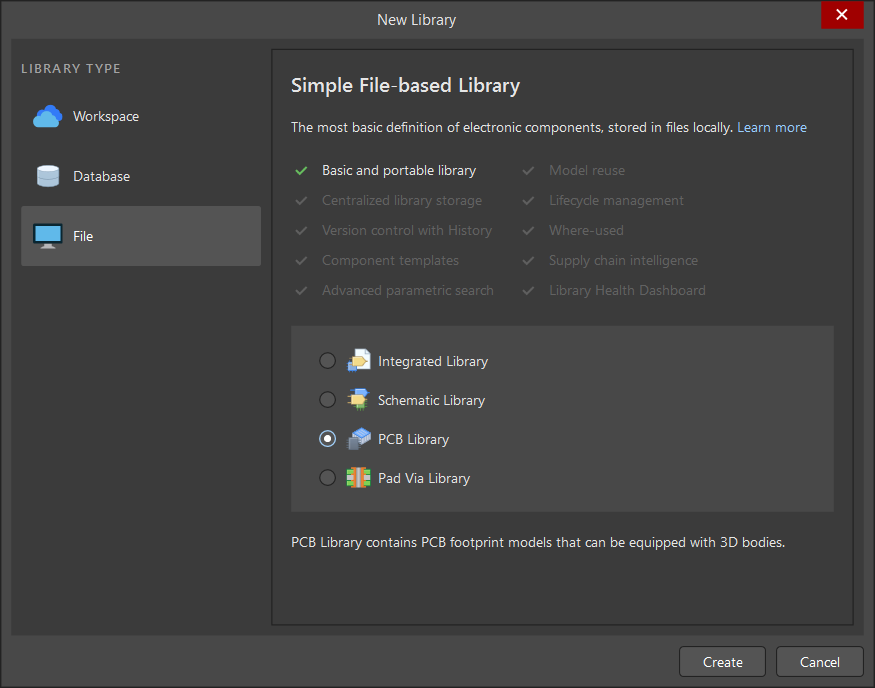
\includegraphics[width=0.7\textwidth]{pictures/ch3.4.png}
                \end{figure}
                Bước 3: Chọn Tools/IPC Compliant Footprint Wizard/Next.
                \begin{figure}[H]
                    \centering
                    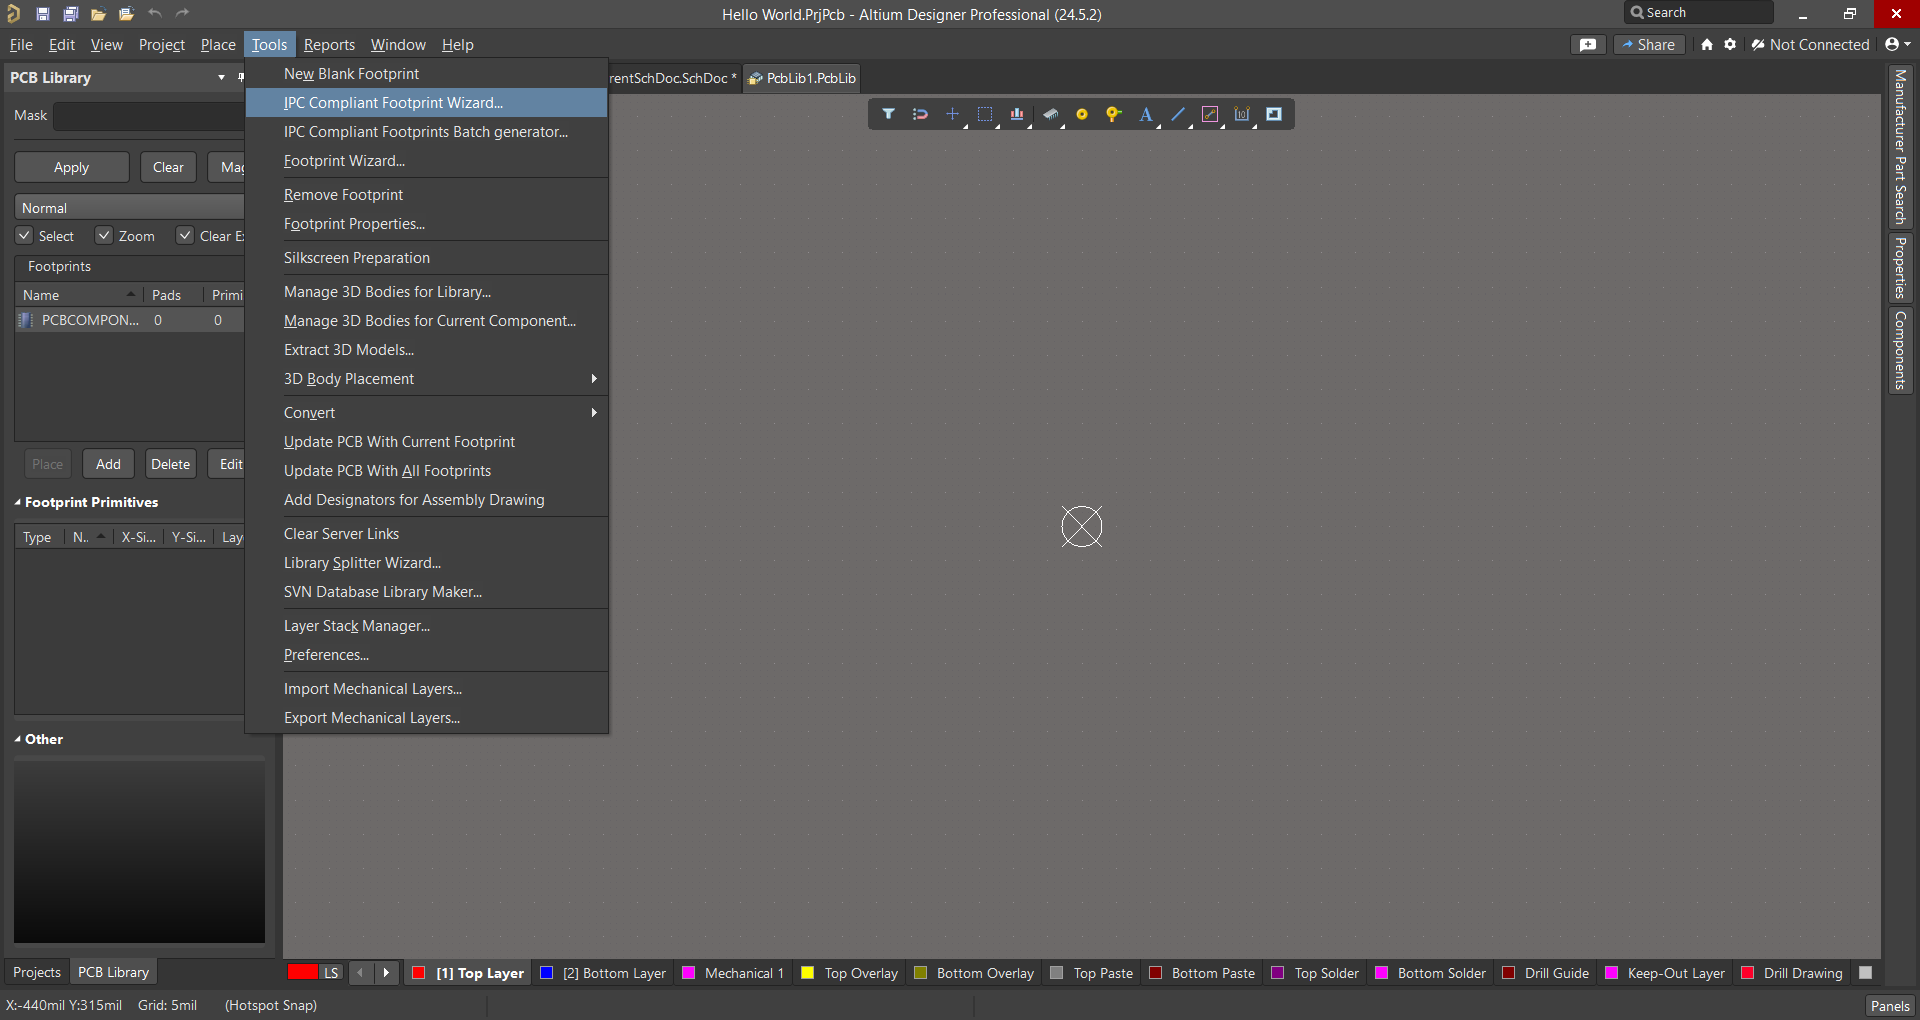
\includegraphics[width=1\textwidth]{pictures/ch3.5.png}
                \end{figure}
                Bước 4: Chọn kiểu chân SOP/TSOP và nhấn NEXT.
                \begin{figure}[H]
                    \centering
                    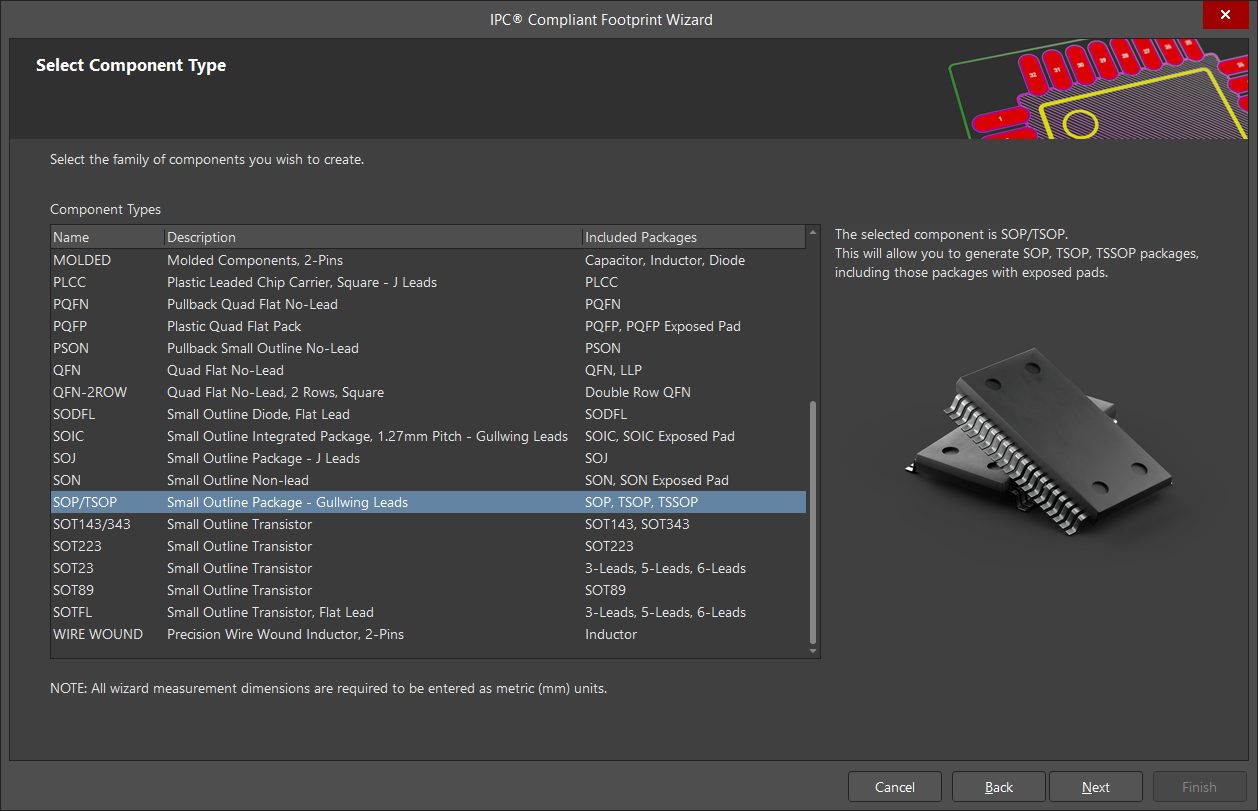
\includegraphics[width=1\textwidth]{pictures/ch3.6.png}
                \end{figure}
                \cleardoublepage
                Bước 5: Đọc datasheet của linh kiện để tìm các thông số thiết kế.
                \begin{figure}[H]
                    \centering
                    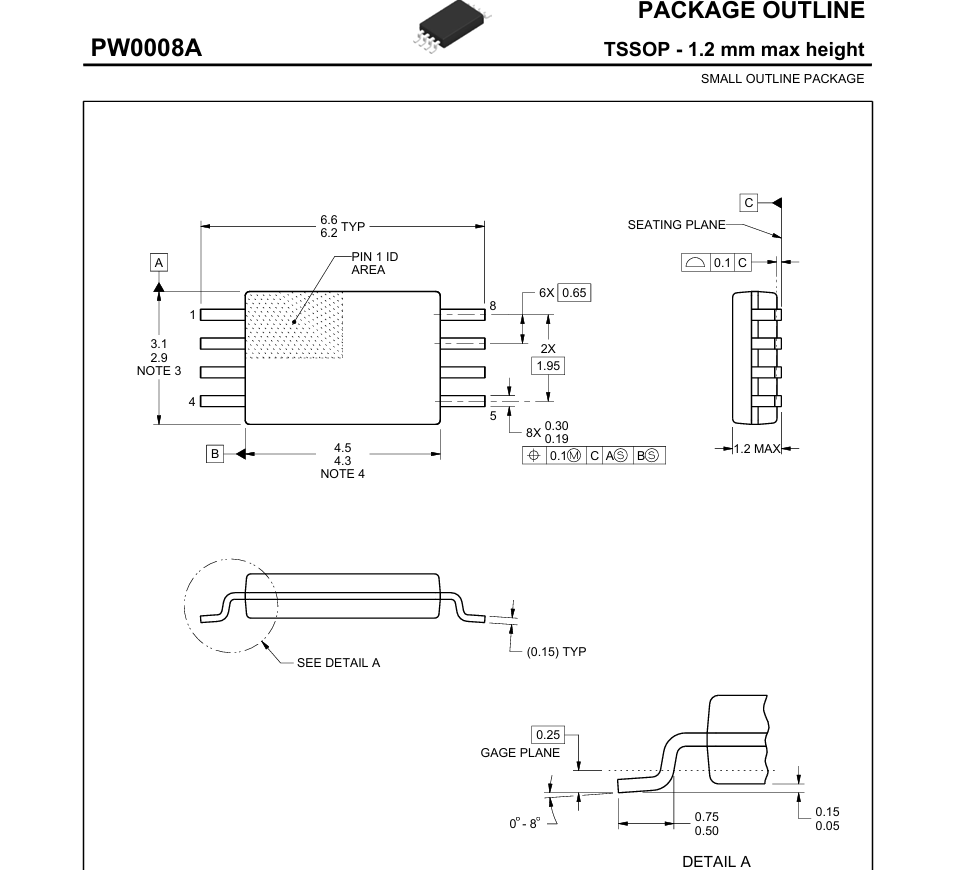
\includegraphics[width=0.9\textwidth]{pictures/ch3.7.png}
                \end{figure}
                Bước 6: Nhập các thông số vào các ô tương ứng và nhấn NEXT.
                \begin{figure}[H]
                    \centering
                    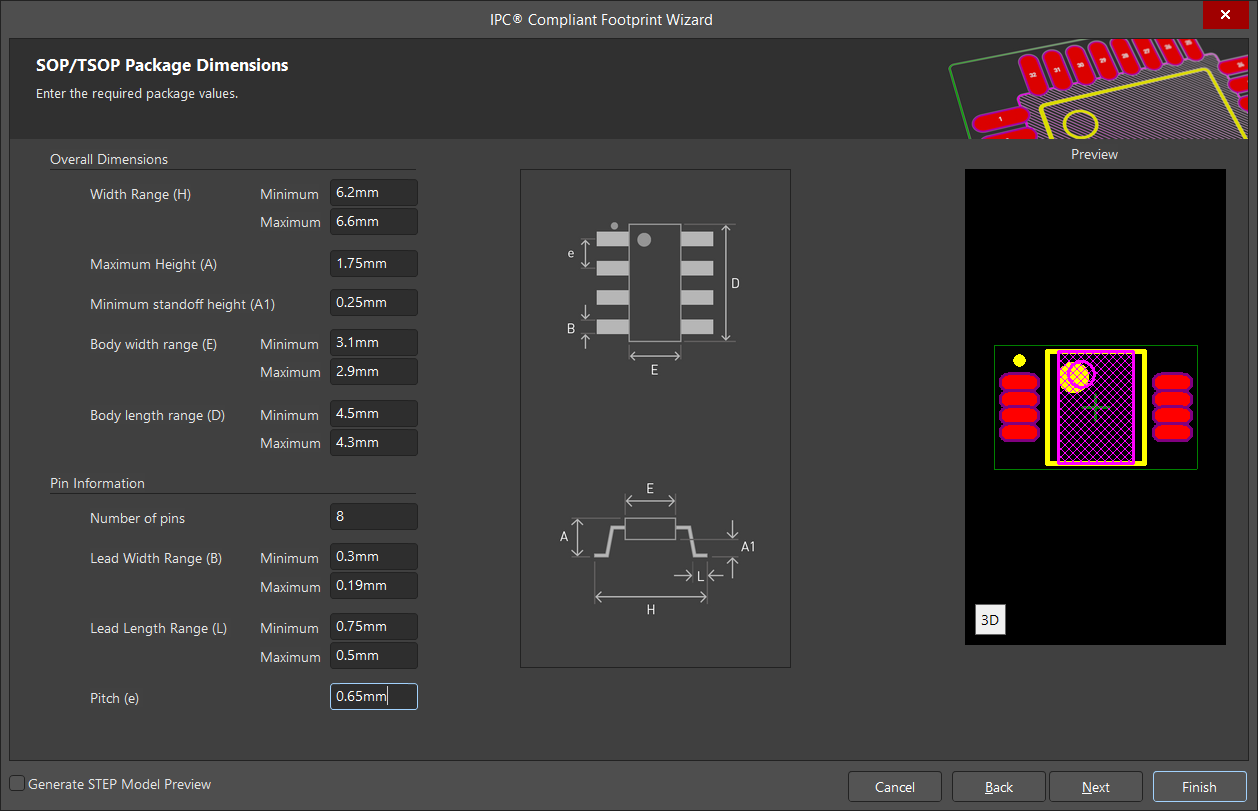
\includegraphics[width=0.8\textwidth]{pictures/ch3.8.png}
                \end{figure}
                Bước 7: Tiếp tục nhấn NEXT cho đến khi đến màn hình lưu và đặt tên.
                \begin{figure}[H]
                    \centering
                    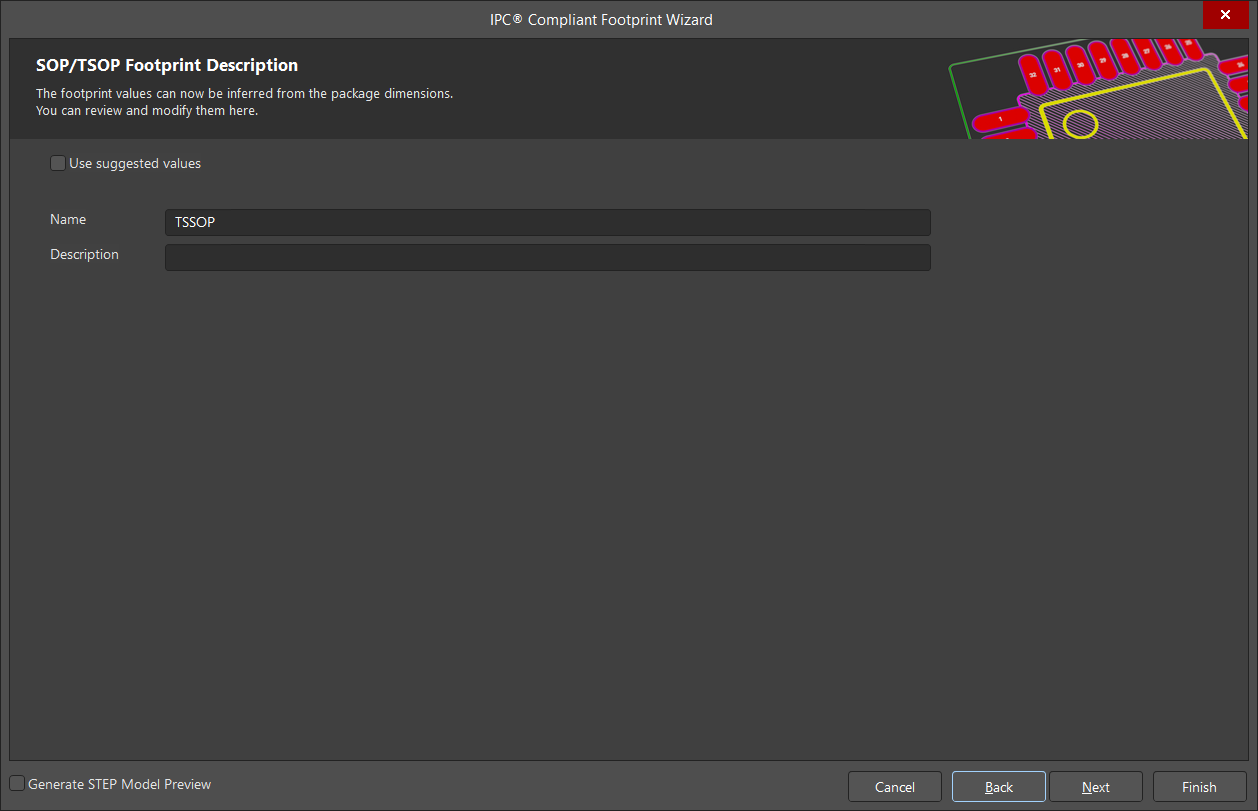
\includegraphics[width=1\textwidth]{pictures/ch3.9.png}
                \end{figure}
                Bước 8: Chọn Produce 3D/STEP model nhấn NEXT và FINISH.
                \begin{figure}[H]
                    \centering
                    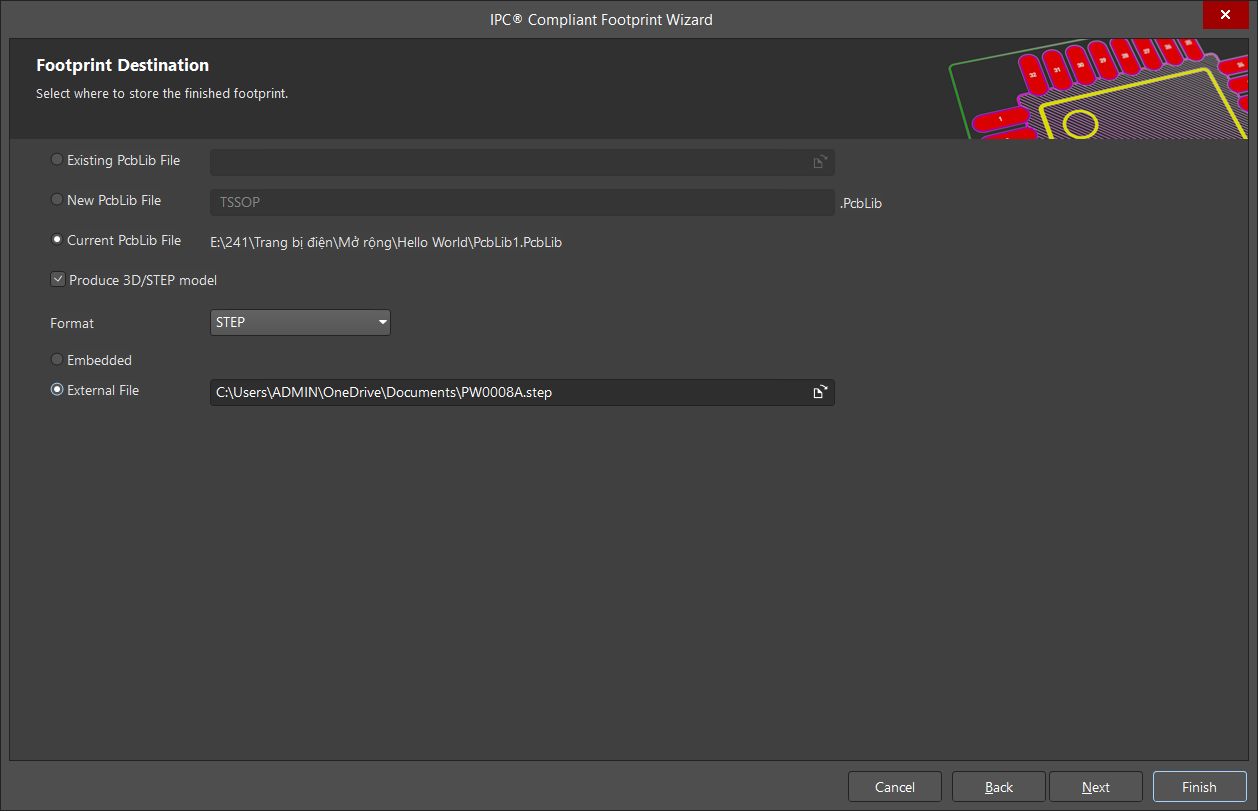
\includegraphics[width=1\textwidth]{pictures/ch3.10.png}
                \end{figure}
                \cleardoublepage
                Bước 9: Hoàn thành việc tạo thư viện footprint cho linh kiện LM358 SOP8.
                \begin{figure}[H]
                    \centering
                    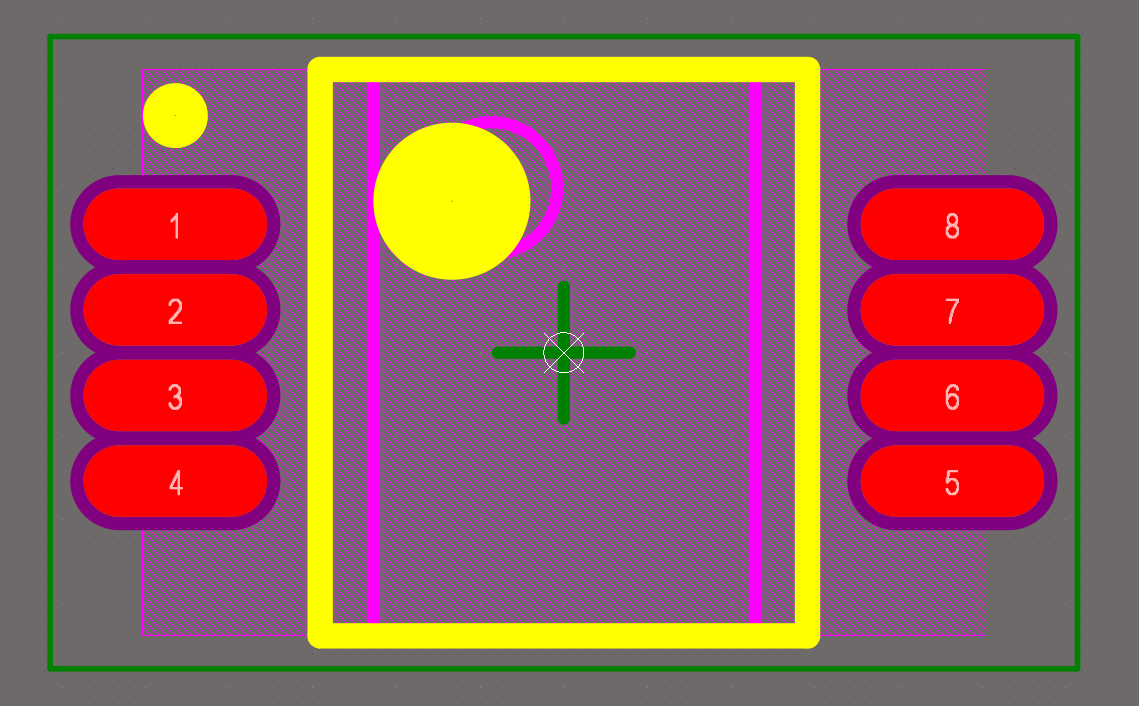
\includegraphics[width=0.9\textwidth]{pictures/ch3.11a.png}
                    \caption{Footprint LM358 SOP8 vừa tạo} 
                \end{figure}
                \begin{figure}[H]
                    \centering
                    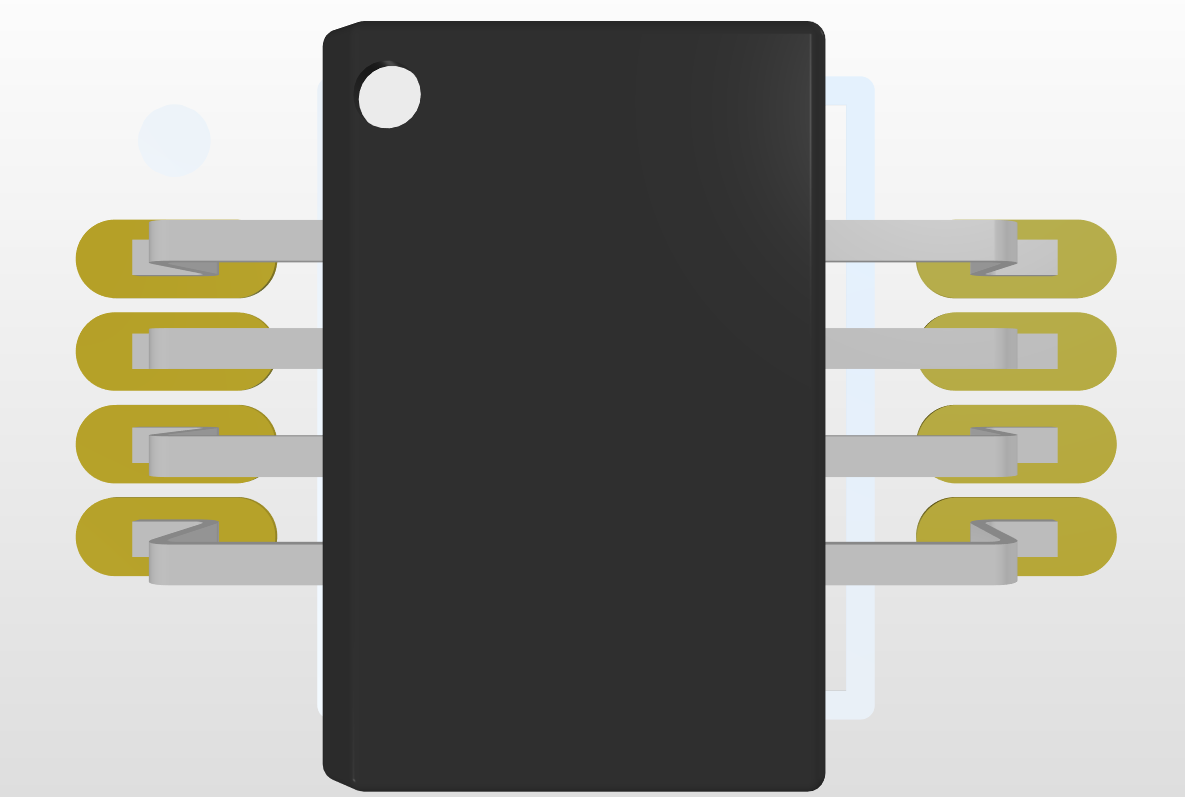
\includegraphics[width=0.9\textwidth]{pictures/ch3.11b.png}
                    \caption{Mô hình PCB 3D LM358 SOP8 vừa tạo}
                \end{figure}
                \cleardoublepage
            \subsection{Add thư viện schematic và thư viện PCB lại với nhau}
                Bước 1: Ở màn hình làm việc của thư viện schematic chọn Add Footprint.
                \begin{figure}[H]
                    \centering
                    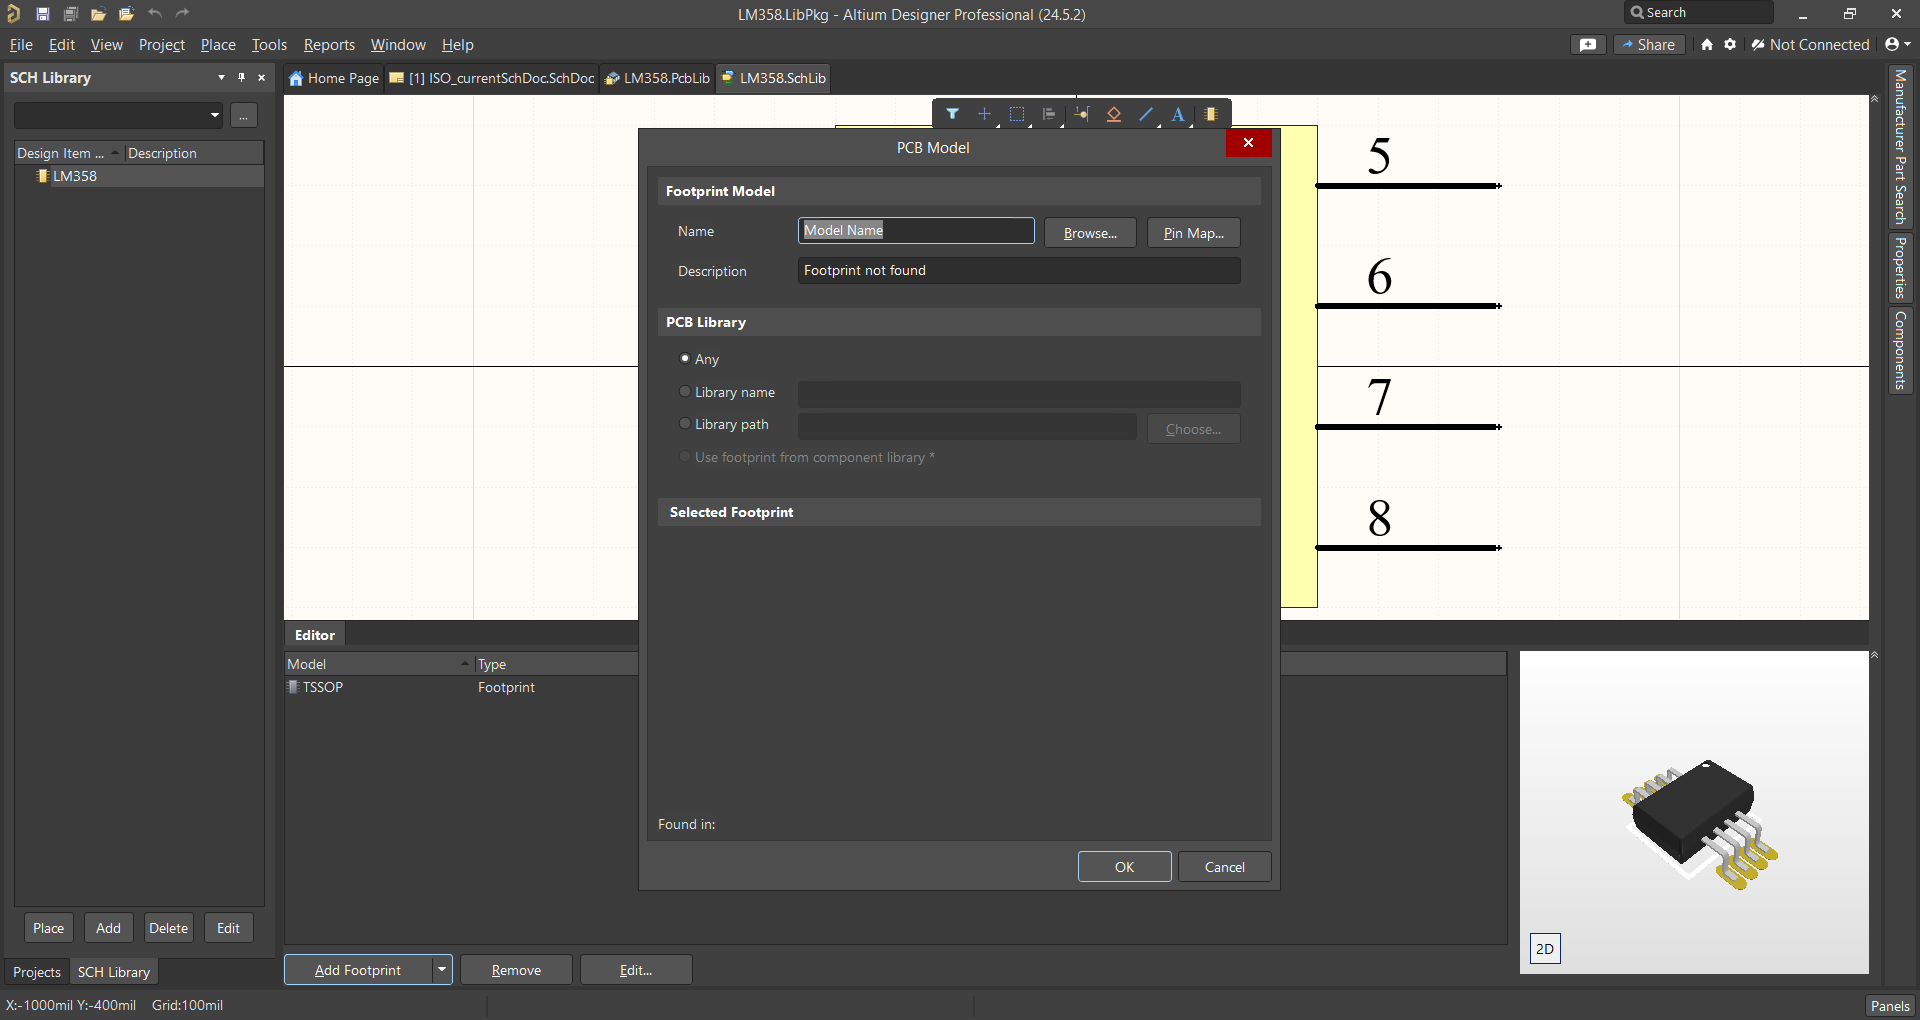
\includegraphics[width=1\textwidth]{pictures/ch3.12.png}
                \end{figure}
                Bước 2: Chọn Browse và chọn thư viện PCB tương ứng và nhấn OK
                \begin{figure}[H]
                    \centering
                    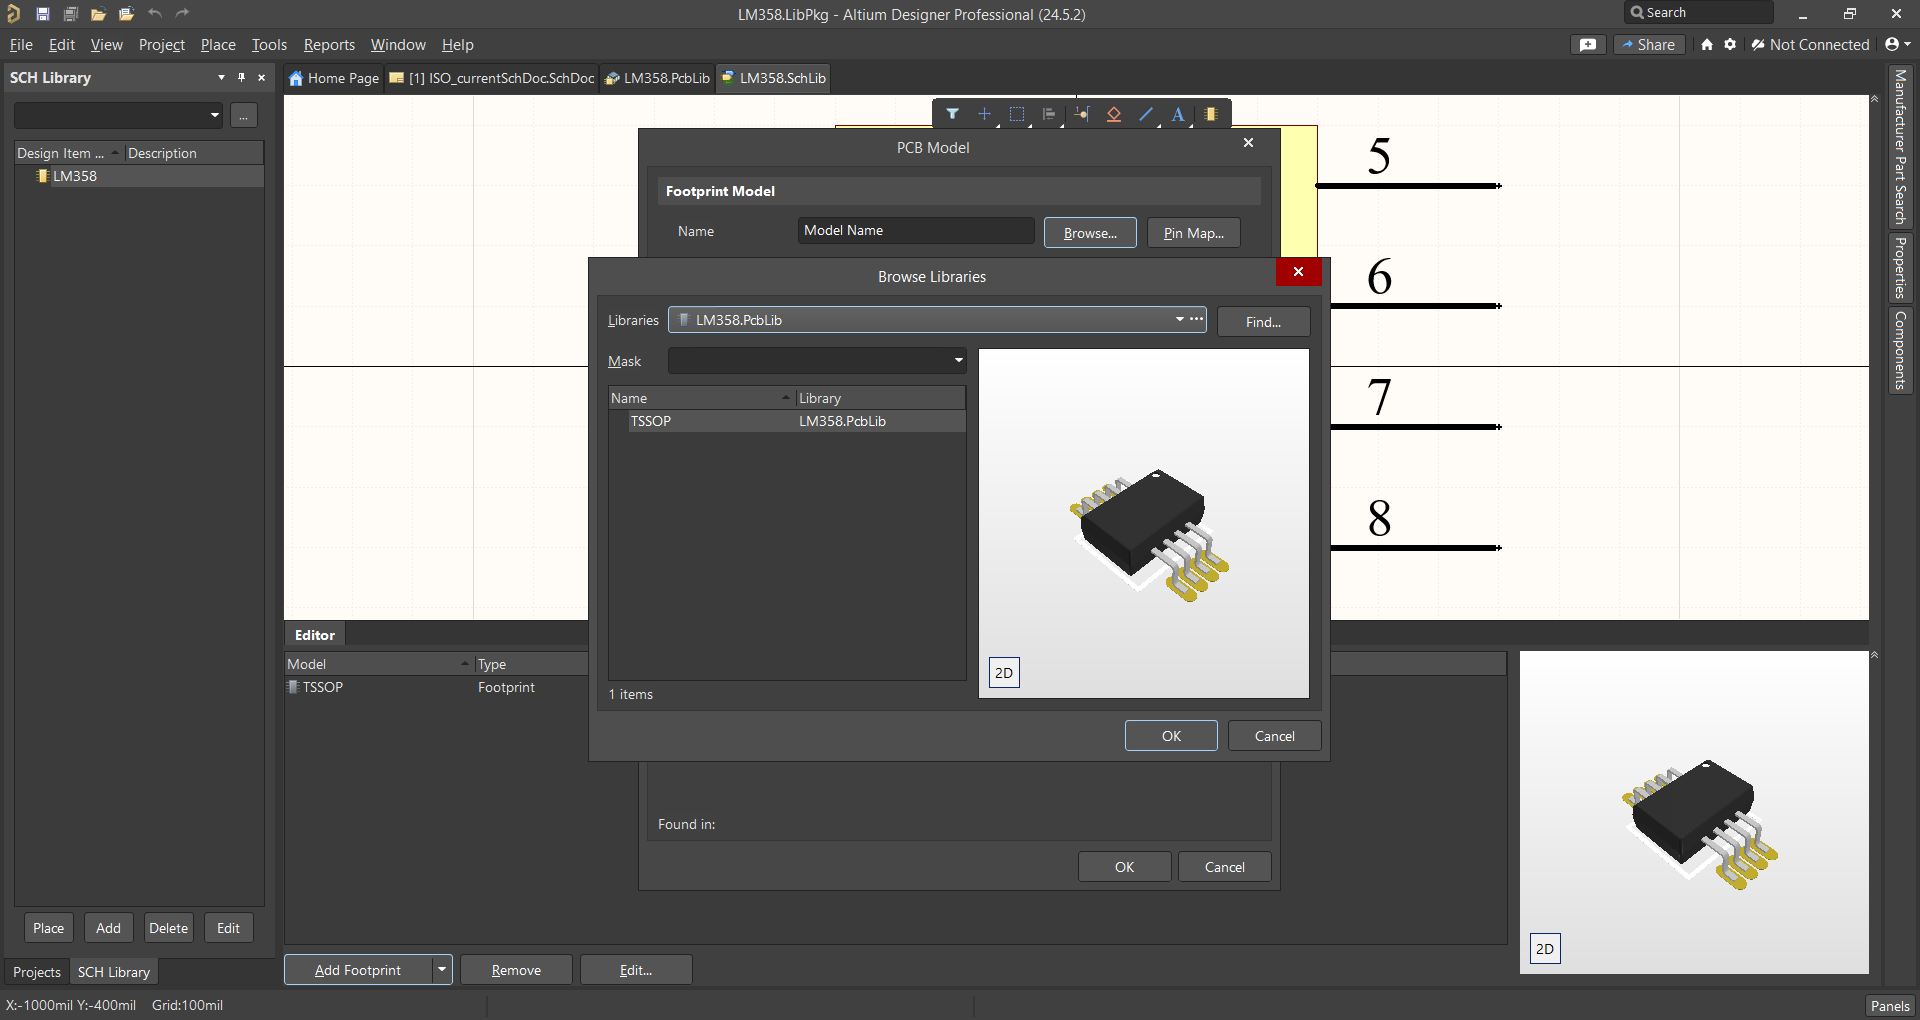
\includegraphics[width=1\textwidth]{pictures/ch3.13.png}
                \end{figure}
                \cleardoublepage
                Bước 3: Vào File/New chọn Library và chọn Integrated Library.
                \begin{figure}[H]
                    \centering
                    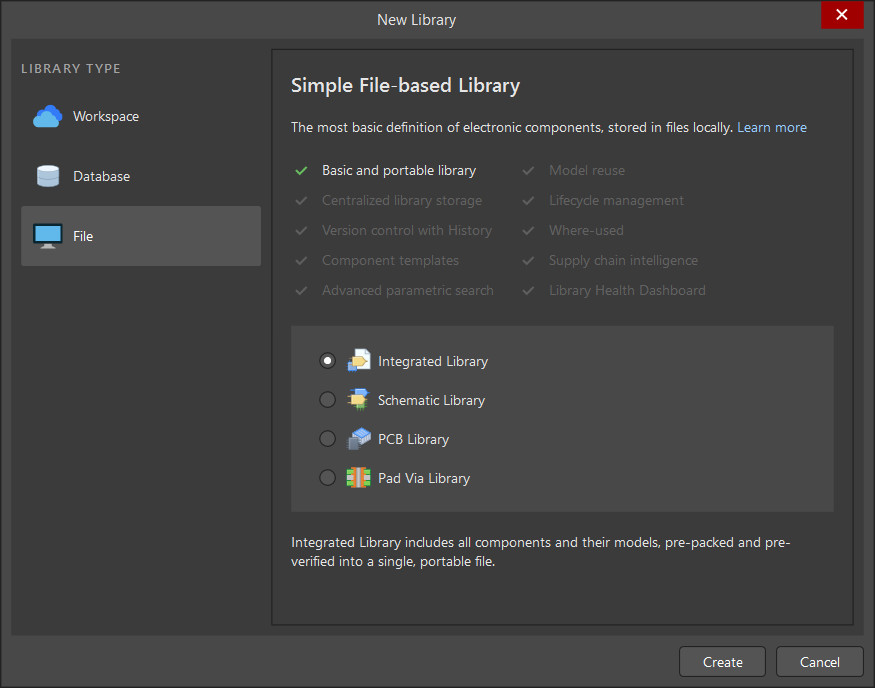
\includegraphics[width=1\textwidth]{pictures/ch3.15.png}
                \end{figure}
                Bước 4: Kéo 2 thư viện schematic và PCB vào Integrated Library vừa tạo và lưu lại. 
                Bước 5: Click chuột phải và chọn Compile Integrated Library.
                \begin{figure}[H]
                    \centering
                    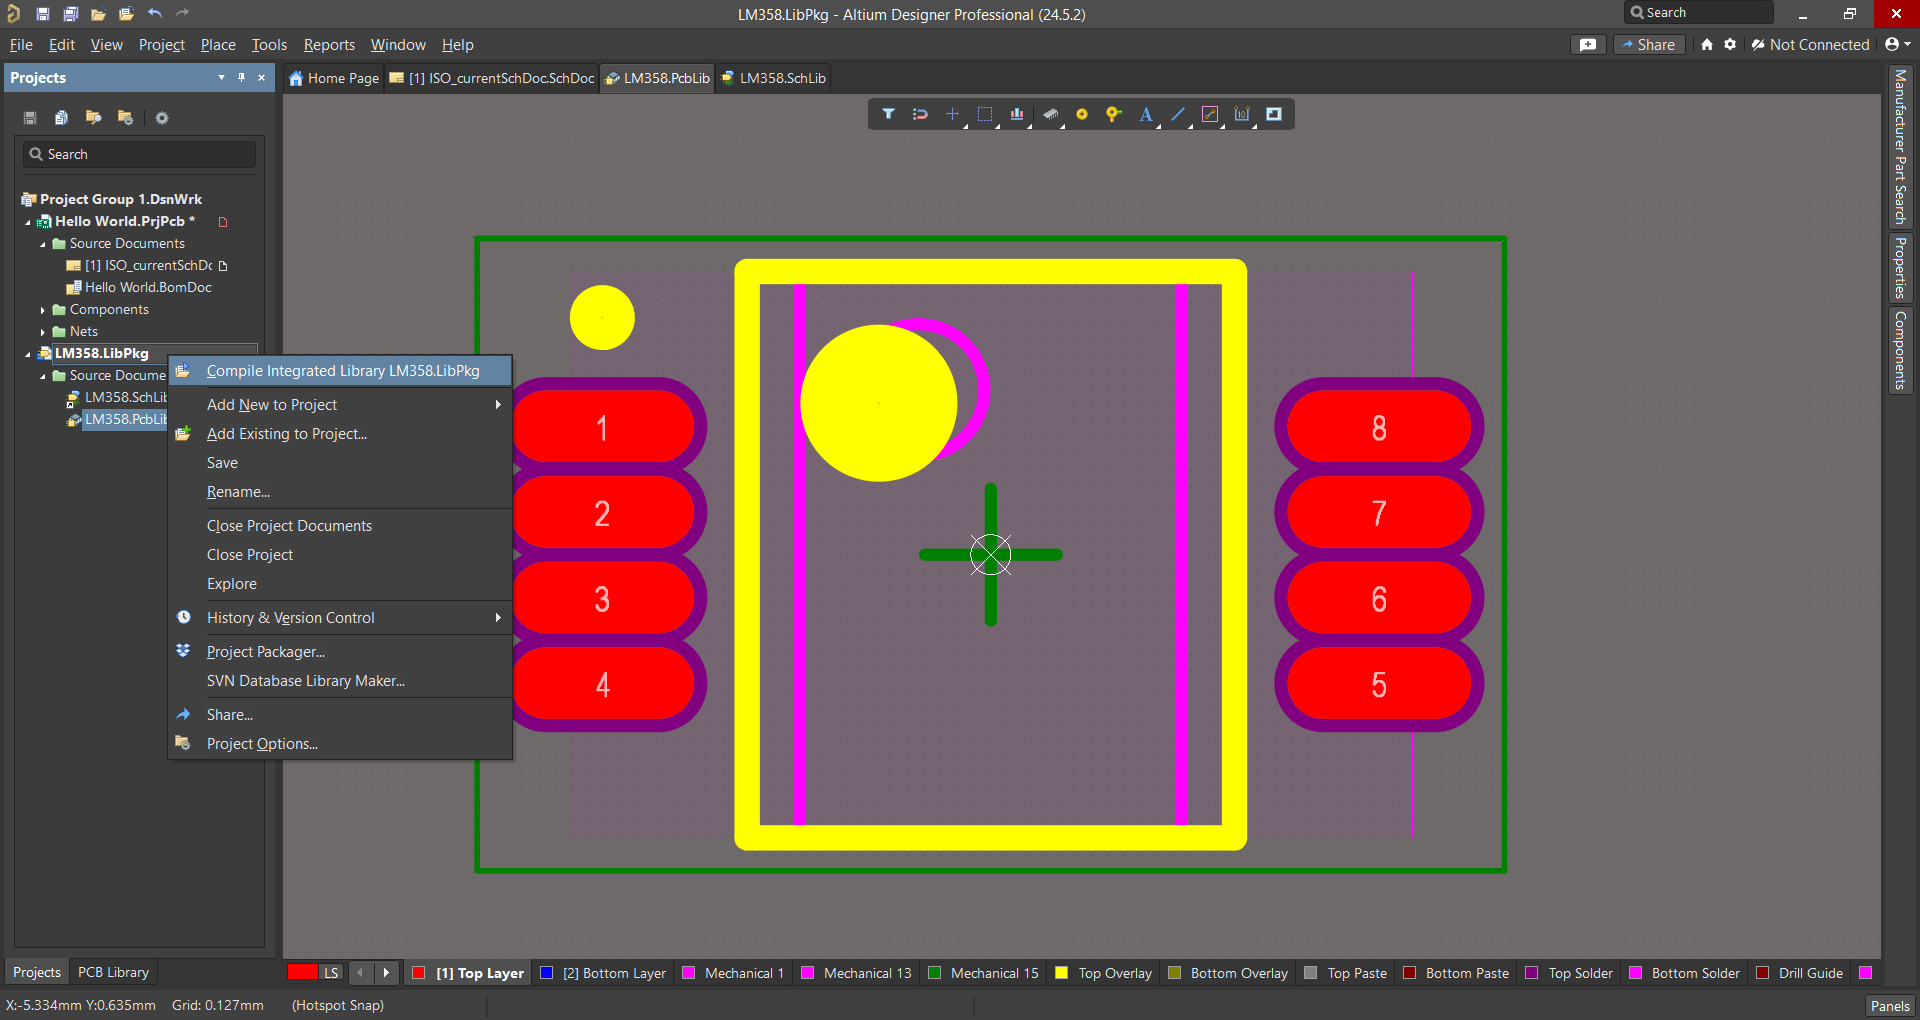
\includegraphics[width=1\textwidth]{pictures/ch3.16.png}
                \end{figure}
                \begin{figure}[H]
                    \centering
                    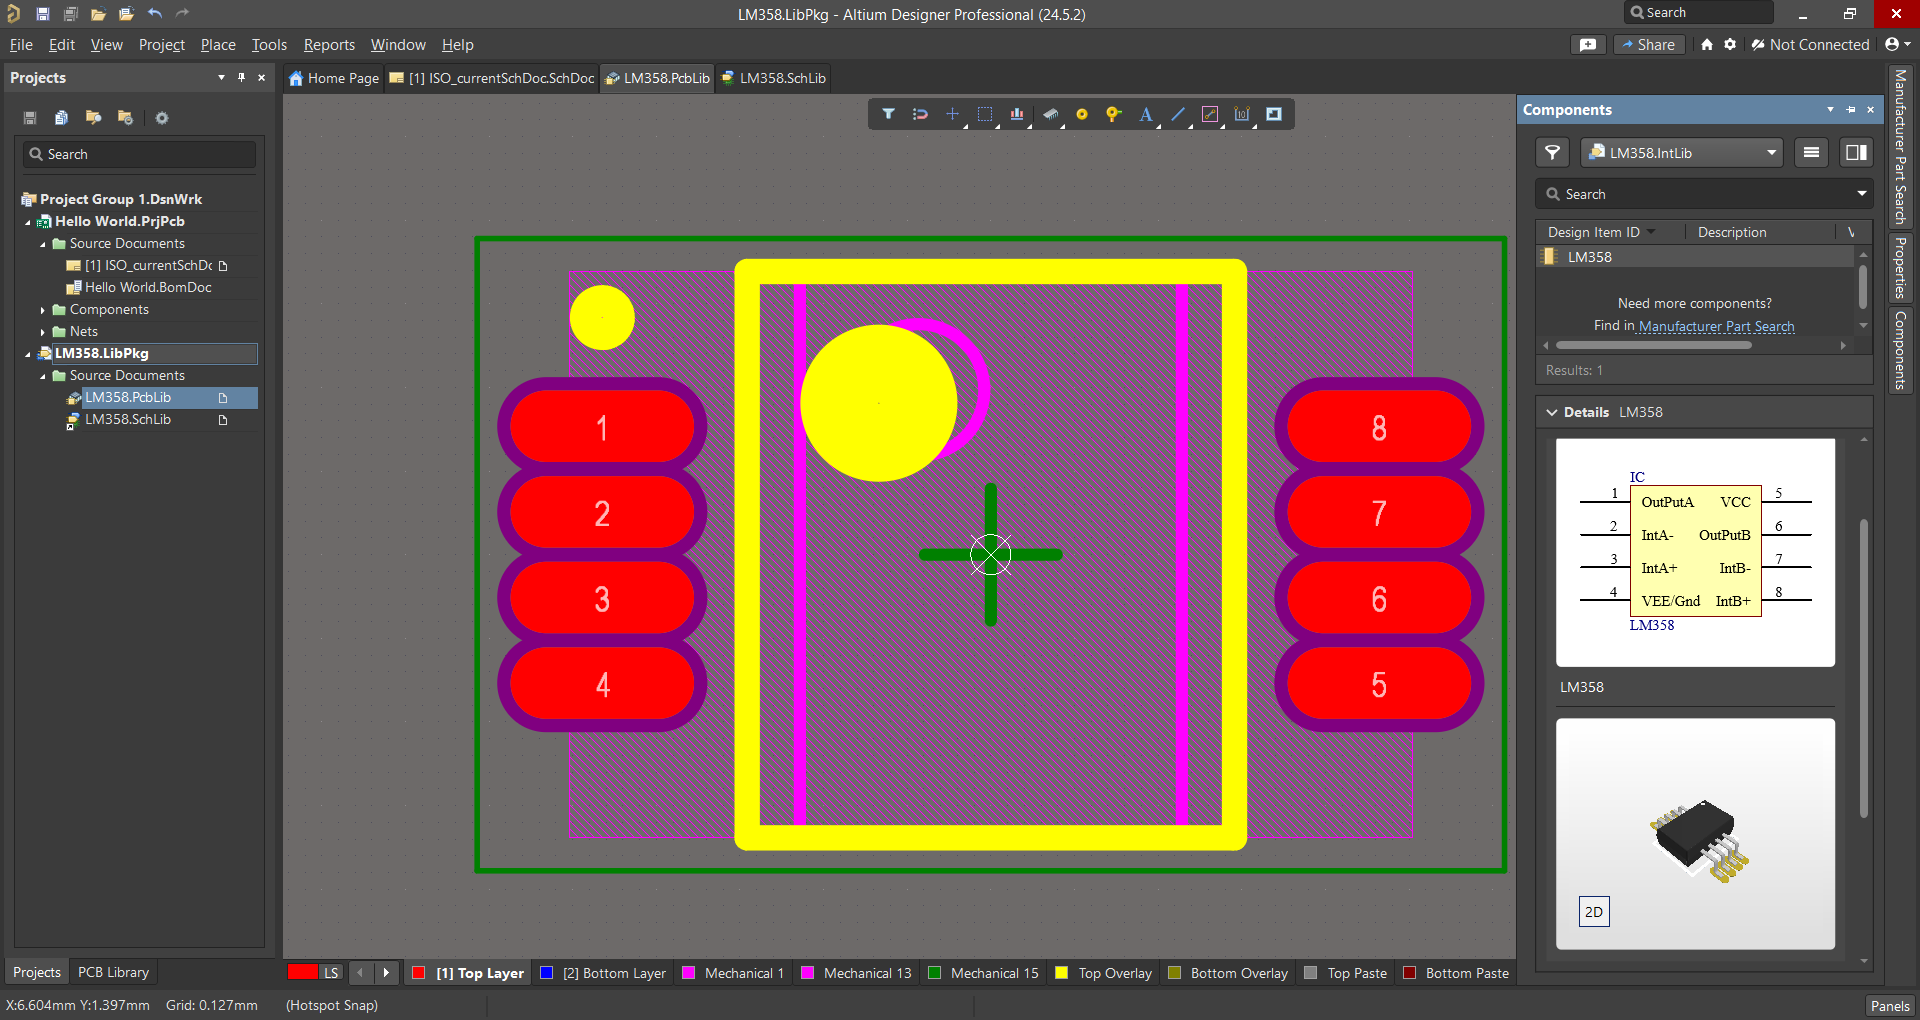
\includegraphics[width=1\textwidth]{pictures/ch3.14.png}
                    \caption{Hoàn tất việc tạo thư viện schematic và PCB 3D cho LM358} 
                \end{figure}
                \cleardoublepage